% Created 2019-07-01 一 04:09
% Intended LaTeX compiler: pdflatex
\documentclass[11pt]{article}
\usepackage[utf8]{inputenc}
\usepackage[T1]{fontenc}
\usepackage{graphicx}
\usepackage{grffile}
\usepackage{longtable}
\usepackage{wrapfig}
\usepackage{rotating}
\usepackage[normalem]{ulem}
\usepackage{amsmath}
\usepackage{textcomp}
\usepackage{amssymb}
\usepackage{capt-of}
\usepackage{hyperref}
\usepackage{minted}
\graphicspath{{../../images/ArtificialIntelligence/}}
% TIPS
% \substack{a\\b} for multiple lines text





% pdfplots will load xolor automatically without option
\usepackage[dvipsnames]{xcolor}

\usepackage{forest}
% two-line text in node by [two \\ lines]
% \begin{forest} qtree, [..] \end{forest}
\forestset{
  qtree/.style={
    baseline,
    for tree={
      parent anchor=south,
      child anchor=north,
      align=center,
      inner sep=1pt,
    }}}
%\usepackage{flexisym}
% load order of mathtools and mathabx, otherwise conflict overbrace

\usepackage{mathtools}
%\usepackage{fourier}
\usepackage{pgfplots}
\usepackage{amsthm}
\usepackage{amsmath}
%\usepackage{unicode-math}
%
\usepackage{commath}
%\usepackage{,  , }
\usepackage{amsfonts}
\usepackage{amssymb}
% importing symbols https://tex.stackexchange.com/questions/14386/importing-a-single-symbol-from-a-different-font
%mathabx change every symbol
% use instead stmaryrd
%\usepackage{mathabx}
\usepackage{stmaryrd}
\usepackage{empheq}
\usepackage{tikz}
\usepackage{tikz-cd}
%\usepackage[notextcomp]{stix}
\usetikzlibrary{arrows.meta}
\usepackage[most]{tcolorbox}
%\utilde
%\usepackage{../../latexpackage/undertilde/undertilde}
% left and right superscript and subscript
\usepackage{actuarialsymbol}
\usepackage{threeparttable}
\usepackage{scalerel,stackengine}
\usepackage{stackrel}
% \stackrel[a]{b}{c}
\usepackage{dsfont}
% text font
\usepackage{newpxtext}
%\usepackage{newpxmath}

%\newcounter{dummy} \numberwithin{dummy}{section}
\newtheorem{dummy}{dummy}[section]
\theoremstyle{definition}
\newtheorem{definition}[dummy]{Definition}
\newtheorem{corollary}[dummy]{Corollary}
\newtheorem{lemma}[dummy]{Lemma}
\newtheorem{proposition}[dummy]{Proposition}
\newtheorem{theorem}[dummy]{Theorem}
\theoremstyle{definition}
\newtheorem{example}[dummy]{Example}
\theoremstyle{remark}
\newtheorem*{remark}{Remark}


\newcommand\what[1]{\ThisStyle{%
    \setbox0=\hbox{$\SavedStyle#1$}%
    \stackengine{-1.0\ht0+.5pt}{$\SavedStyle#1$}{%
      \stretchto{\scaleto{\SavedStyle\mkern.15mu\char'136}{2.6\wd0}}{1.4\ht0}%
    }{O}{c}{F}{T}{S}%
  }
}

\newcommand\wtilde[1]{\ThisStyle{%
    \setbox0=\hbox{$\SavedStyle#1$}%
    \stackengine{-.1\LMpt}{$\SavedStyle#1$}{%
      \stretchto{\scaleto{\SavedStyle\mkern.2mu\AC}{.5150\wd0}}{.6\ht0}%
    }{O}{c}{F}{T}{S}%
  }
}

\newcommand\wbar[1]{\ThisStyle{%
    \setbox0=\hbox{$\SavedStyle#1$}%
    \stackengine{.5pt+\LMpt}{$\SavedStyle#1$}{%
      \rule{\wd0}{\dimexpr.3\LMpt+.3pt}%
    }{O}{c}{F}{T}{S}%
  }
}

\newcommand{\bl}[1] {\boldsymbol{#1}}
\newcommand{\Wt}[1] {\stackrel{\sim}{\smash{#1}\rule{0pt}{1.1ex}}}
\newcommand{\wt}[1] {\widetilde{#1}}
\newcommand{\tf}[1] {\textbf{#1}}


%For boxed texts in align, use Aboxed{}
%otherwise use boxed{}

\DeclareMathSymbol{\widehatsym}{\mathord}{largesymbols}{"62}
\newcommand\lowerwidehatsym{%
  \text{\smash{\raisebox{-1.3ex}{%
    $\widehatsym$}}}}
\newcommand\fixwidehat[1]{%
  \mathchoice
    {\accentset{\displaystyle\lowerwidehatsym}{#1}}
    {\accentset{\textstyle\lowerwidehatsym}{#1}}
    {\accentset{\scriptstyle\lowerwidehatsym}{#1}}
    {\accentset{\scriptscriptstyle\lowerwidehatsym}{#1}}
}

\usepackage{graphicx}
    
% text on arrow for xRightarrow
\makeatletter
%\newcommand{\xRightarrow}[2][]{\ext@arrow 0359\Rightarrowfill@{#1}{#2}}
\makeatother


\newcommand{\dom}[1]{%
\mathrm{dom}{(#1)}
}

% Roman numerals
\makeatletter
\newcommand*{\rom}[1]{\expandafter\@slowromancap\romannumeral #1@}
\makeatother

\def \fR {\mathfrak{R}}
\def \bx {\boldsymbol{x}}
\def \bz {\boldsymbol{z}}
\def \ba {\boldsymbol{a}}
\def \bh {\boldsymbol{h}}
\def \bo {\boldsymbol{o}}
\def \bU {\boldsymbol{U}}
\def \bc {\boldsymbol{c}}
\def \bV {\boldsymbol{V}}
\def \bI {\boldsymbol{I}}
\def \bK {\boldsymbol{K}}
\def \bt {\boldsymbol{t}}
\def \bb {\boldsymbol{b}}
\def \bA {\boldsymbol{A}}
\def \bX {\boldsymbol{X}}
\def \bu {\boldsymbol{u}}
\def \bS {\boldsymbol{S}}
\def \bZ {\boldsymbol{Z}}
\def \bz {\boldsymbol{z}}
\def \by {\boldsymbol{y}}
\def \bw {\boldsymbol{w}}
\def \bT {\boldsymbol{T}}
\def \bF {\boldsymbol{F}}
\def \bS {\boldsymbol{S}}
\def \bm {\boldsymbol{m}}
\def \bW {\boldsymbol{W}}
\def \bR {\boldsymbol{R}}
\def \bQ {\boldsymbol{Q}}
\def \bS {\boldsymbol{S}}
\def \bP {\boldsymbol{P}}
\def \bT {\boldsymbol{T}}
\def \bY {\boldsymbol{Y}}
\def \bH {\boldsymbol{H}}
\def \bB {\boldsymbol{B}}
\def \blambda {\boldsymbol{\lambda}}
\def \bPhi {\boldsymbol{\Phi}}
\def \btheta {\boldsymbol{\theta}}
\def \bTheta {\boldsymbol{\Theta}}
\def \bmu {\boldsymbol{\mu}}
\def \bphi {\boldsymbol{\phi}}
\def \bSigma {\boldsymbol{\Sigma}}
\def \lb {\left\{}
\def \rb {\right\}}
\def \la {\langle}
\def \ra {\rangle}
\def \caln {\mathcal{N}}
\def \dissum {\displaystyle\Sigma}
\def \dispro {\displaystyle\prod}
\def \E {\mathbb{E}}
\def \Q {\mathbb{Q}}
\def \N {\mathbb{N}}
\def \V {\mathbb{V}}
\def \R {\mathbb{R}}
\def \P {\mathbb{P}}
\def \A {\mathbb{A}}
\def \Z {\mathbb{Z}}
\def \I {\mathbb{I}}
\def \C {\mathbb{C}}
\def \cala {\mathcal{A}}
\def \calb {\mathcal{B}}
\def \calq {\mathcal{Q}}
\def \calp {\mathcal{P}}
\def \cals {\mathcal{S}}
\def \calg {\mathcal{G}}
\def \caln {\mathcal{N}}
\def \calr {\mathcal{R}}
\def \calm {\mathcal{M}}
\def \calc {\mathcal{C}}
\def \calf {\mathcal{F}}
\def \calk {\mathcal{K}}
\def \call {\mathcal{L}}
\def \calu {\mathcal{U}}
\def \bcup {\bigcup}


\def \uin {\underline{\in}}
\def \oin {\overline{\in}}
\def \uR {\underline{R}}
\def \oR {\overline{R}}
\def \uP {\underline{P}}
\def \oP {\overline{P}}

\def \Ra {\Rightarrow}

\def \e {\enspace}

\def \sgn {\operatorname{sgn}}
\def \gen {\operatorname{gen}}
\def \ker {\operatorname{ker}}
\def \im {\operatorname{im}}

\def \tril {\triangleleft}

% \varprod
\DeclareSymbolFont{largesymbolsA}{U}{txexa}{m}{n}
\DeclareMathSymbol{\varprod}{\mathop}{largesymbolsA}{16}

% \bigtimes
\DeclareFontFamily{U}{mathx}{\hyphenchar\font45}
\DeclareFontShape{U}{mathx}{m}{n}{
      <5> <6> <7> <8> <9> <10>
      <10.95> <12> <14.4> <17.28> <20.74> <24.88>
      mathx10
      }{}
\DeclareSymbolFont{mathx}{U}{mathx}{m}{n}
\DeclareMathSymbol{\bigtimes}{1}{mathx}{"91}
% \odiv
\DeclareFontFamily{U}{matha}{\hyphenchar\font45}
\DeclareFontShape{U}{matha}{m}{n}{
      <5> <6> <7> <8> <9> <10> gen * matha
      <10.95> matha10 <12> <14.4> <17.28> <20.74> <24.88> matha12
      }{}
\DeclareSymbolFont{matha}{U}{matha}{m}{n}
\DeclareMathSymbol{\odiv}         {2}{matha}{"63}


\newcommand\subsetsim{\mathrel{%
  \ooalign{\raise0.2ex\hbox{\scalebox{0.9}{$\subset$}}\cr\hidewidth\raise-0.85ex\hbox{\scalebox{0.9}{$\sim$}}\hidewidth\cr}}}
\newcommand\simsubset{\mathrel{%
  \ooalign{\raise-0.2ex\hbox{\scalebox{0.9}{$\subset$}}\cr\hidewidth\raise0.75ex\hbox{\scalebox{0.9}{$\sim$}}\hidewidth\cr}}}

\newcommand\simsubsetsim{\mathrel{%
  \ooalign{\raise0ex\hbox{\scalebox{0.8}{$\subset$}}\cr\hidewidth\raise1ex\hbox{\scalebox{0.75}{$\sim$}}\hidewidth\cr\raise-0.95ex\hbox{\scalebox{0.8}{$\sim$}}\cr\hidewidth}}}
\newcommand{\stcomp}[1]{{#1}^{\mathsf{c}}}


\author{wu}
\date{\today}
\title{Artificial Intelligence}
\hypersetup{
 pdfauthor={wu},
 pdftitle={Artificial Intelligence},
 pdfkeywords={},
 pdfsubject={},
 pdfcreator={Emacs 26.2 (Org mode 9.2.4)}, 
 pdflang={English}}
\begin{document}

\maketitle
\tableofcontents

\section{scope [57\%]}
\label{sec:org4262ac7}
\begin{itemize}
\item[{$\boxtimes$}] uninformed search and informed search
\item[{$\boxtimes$}] adversarial search: minimax, evaluation functions, alpha-beta search,
stochasitc search
\item[{$\boxminus$}] Basic concept for Statistical Learning and modeling
\begin{itemize}
\item[{$\boxtimes$}] Probability Theory
\item[{$\square$}] Model selection
\item[{$\boxtimes$}] The curse of Dimensionality
\item[{$\boxtimes$}] Decision Theory
\item[{$\boxtimes$}] Information Theory
\item[{$\boxtimes$}] Probability Distribution
\end{itemize}
\item[{$\boxtimes$}] Supervised Learning
\begin{itemize}
\item[{$\boxtimes$}] Linear model for regression
\item[{$\boxtimes$}] Linear basis function models
\item[{$\boxtimes$}] Linear model for classification
\item[{$\boxtimes$}] Adaboosting
\end{itemize}
\item[{$\boxtimes$}] Unsupervised Learning
\begin{itemize}
\item[{$\boxtimes$}] K-means Clustering
\item[{$\boxtimes$}] GMM \& EM algorithm
\item[{$\boxtimes$}] Principal Component Analysis
\end{itemize}
\item[{$\square$}] Deep Learning
\begin{itemize}
\item[{$\square$}] Stochastic Gradient Descent
\item[{$\square$}] Backpropagation
\item[{$\square$}] Feedforward Neural Network
\item[{$\square$}] Convolutional Neural Networks
\item[{$\square$}] Deep learning in CV (localization)
\item[{$\square$}] Recurrent Neural Network (LSTM, GRU)
\end{itemize}
\item[{$\square$}] Reinforcement learning
\begin{itemize}
\item[{$\square$}] Reinforcement learning
\item[{$\square$}] Markov Decision Process
\item[{$\square$}] Value-based Optimization; Q-learning
\end{itemize}
\end{itemize}
\section{Basic concepts for filling in blanks or single choice [45\%]}
\label{sec:org82e9675}
\begin{itemize}
\item[{$\boxtimes$}] Uninformed search (blind search)
\begin{itemize}
\item[{$\boxtimes$}] Problem definition, initial state, actions, transition model, goal
test, path cost, step cost, frontier (open list), loopy path, explored set
(closed set), tree-search, graph-search, queue, completeness, optimality,
time complexity, space complexity
\item[{$\boxtimes$}] Breadth-first search (BFS)
\item[{$\boxtimes$}] Depth-first search (DFS)
\item[{$\boxtimes$}] Uniform-cost search (UCS), Depth-limited search (DLS), iterative
deepening search (IDS)
\end{itemize}
\item[{$\boxtimes$}] informed (heuristic) search
\begin{itemize}
\item[{$\boxtimes$}] Heuristic function h(n), evaluation function f(n), path cost g(n)
\item[{$\boxtimes$}] Best-first search: use f(n) instead of g(n)
\item[{$\boxtimes$}] Greedy best-first search: f(n) = h(n)
\item[{$\boxtimes$}] A* search: f(n) = g(n) + h(n), it is identical to Uniform-Cost-Search
except that A* uses g+h instead of g
\item[{$\boxtimes$}] Conditions for A* optimality: Admissibility and Consistency

\textbf{Noteeeeeeeeee}
\end{itemize}
\item[{$\boxtimes$}] Adversarial search
\begin{itemize}
\item[{$\boxtimes$}] Minimax search: min node, max node, utility
\item[{$\boxtimes$}] Alpha-Beta Pruning Search: alpha value, beta value, pruning

\textbf{STARRRRRRRRRRRRRRRRR}
\end{itemize}
\item[{$\boxtimes$}] Uninformed search vs. informed search
\item[{$\square$}] common concepts
\begin{itemize}
\item[{$\square$}] train set, test set, validation set, S-fold cross-validation
\item[{$\square$}] model selection, model comparison
\item[{$\square$}] over-fitting, under-fitting, SSE error, RMS error, how to control over-fitting,
\item[{$\square$}] penalty term, regularization, shrinkage methods, curse of dimensionality,
\end{itemize}
\item[{$\boxminus$}] probability theory
\begin{itemize}
\item[{$\boxtimes$}] marginal, joint distribution, conditional probability, PDF, CDF, expectation, variance,
covariance and their properties
\item[{$\boxtimes$}] i.i.d, MLE- Maximum Likelihood Estimation, MAPMaximum posterior, log
likelihood, Gaussian distribution, Mahalanobis distance,
\item[{$\square$}] independent parameters, conjugate prior, kernel density estimator, KNN density
estimator, KNN classifier,
\end{itemize}
\item[{$\boxtimes$}] Information theory and decision theory
\begin{itemize}
\item[{$\boxtimes$}] entropy, cross entropy, relative entropy (Kullback-Leibler divergence, KL divergence),
mutual information
\item[{$\boxtimes$}] Naïve Bayes classifier, decision rule, reject option
\end{itemize}
\item[{$\square$}] Supervised learning
\begin{itemize}
\item[{$\square$}] Regression: linear regression, linear basis function model, ridge regression,
stochastic gradient descent, weight decay, sparse model, lasso,
bias-variance tradeoff,
\item[{$\square$}] Classification: linear separable, decision regions, decision boundaries,
decision surfaces, 1-of-K code (one hot code), Least-squares approach,
Fisher’s linear discriminant, the perceptron algorithm of Rosenblatt, loss
function, hinge loss, The Fisher’s criterion, Generalized Rayleigh
quotient, Perceptron criterion, probabilistic generative model, logistic
nsigmoid function, logit function, softmax function, probabilistic
discriminative model, logistic regression
\item[{$\square$}] Boosting: adaboost, committees, bagging, algorithm,
\end{itemize}
\item[{$\square$}] Unsupervised learning
\begin{itemize}
\item[{$\square$}] Clustering: partitional clustering, hierarchical clustering, k-means,
k-medoids, limitation, MoG, E-step, M-step
\item[{$\square$}] Dimensionality Reduction: latent factors, correlation, Pearson
correlation coefficient, correlation vs. independence, PCA, eigenface
\end{itemize}
\item[{$\square$}] deep learning
\begin{itemize}
\item[{$\square$}] NN: activation function, neuron model, ReLU, TanH, Sigmoid,
feed-forward NN, fully-connected layer, hidden layer, multilayer
perceptron, gradient descent, SGD, SGD+ADAM, backpropagation, chain rule,
computational graph, automatic differentiation, forward
computation+backpropagatio
\item[{$\square$}] CNN: AlexNet, VGG, GoogLeNet, ResNet, ImageNet, convolutional layer,
receptive field, convolutional kernel / convolutional filter, stride,
padding, zero padding, activation / feature map, pooling layer, max
pooling, average pooling / L2-norm pooling, downsampling, upsampling,
batch normalization, FC layer, Fully convolutional networks, data
augmentation, dropout, dropconnect, transfer learning, localization,
object detection
\item[{$\square$}] RNN: encoder-decoder sequence-to-sequence architecture, LSTM, GRU,
image captioning, sentiment classification, machine translation, video
classification on frame level, visual question answering, truncated
backpropagation through time
\end{itemize}
\item[{$\square$}] reinforcement learning
\begin{itemize}
\item[{$\square$}] Policy, reward, cumulative reward, return, discount factor, value,
Markov process, Markov reward process, MDP-Markov decision process,
episodic, state transition probability matrix, value function,
action-value/Q-value function, QLearning, policy improvement, policy
evaluation, bellman equation, dynamic programming, Monte Carlo sampling,
Temporal Difference
\end{itemize}
\end{itemize}

\section{solving problems by search}
\label{sec:org2337cbb}
\textbf{problem-solving agent}
\begin{itemize}
\item \textbf{goal}
\item \textbf{goal information} is the 1st step in problem-solving, based on the
current situation and the agent’s performance measure
\item \textbf{problem formulation} is the process of deciding what actions and
states to consider, given a goal
\item \textbf{search}
\item \textbf{execution phase}
\end{itemize}


formulate—search—execution


type of search
\begin{itemize}
\item \textbf{uninformed search algorithms}

algorithms that are given no information about the problem other
than its definition. Although some of these algorithms can solve
any solvable problem, none of them can do so efficiently
\item \textbf{informed search algorithms}
\end{itemize}


The types of Problem-solving by Search
\begin{itemize}
\item Deterministic, fully observable

Agent knows exactly which state it will be in

solution is a sequence
\item non-observable

Agent may have no idea where it is

solution (if any) is a sequence
\item Nondeterministic and/or partially observable

percepts provide new information about current state

solution is a tree or policy

often interleave search, execution
\item Unknown state space
\end{itemize}


Some assumptions about environment
\begin{itemize}
\item \textbf{observable}
\item \textbf{discrete}: the environment is discrete
\item \textbf{known}: the agent knows which states are reached by each action
\item \textbf{deterministic}: each action has exactly one outcome
\end{itemize}


\textbf{Problem definition}
\begin{enumerate}
\item \textbf{Initial state}
\item \textbf{actions}
\item \textbf{Transition model}
\item \textbf{goal test}: determines whether a given state is a goal state
\item \textbf{path cost}: a function that assigns a numeric cost to each path
\end{enumerate}


A solution is an \textbf{action sequence}, so search algorithms work
by considering various possible action sequences.


Given a search tree, the set of all leaf nodes available for expansion at any
given point is called the \textbf{frontier(open list)}. \textbf{Search strategy}


queues: FIFO queue, LIFO queue (stack), priority queue


Measuring problem-solving performance: 
\begin{itemize}
\item completeness: Does it always find a solution
\item optimality: How long does it take?
\item time complexity
\item space complexity
\end{itemize}


\textbf{uninformd search}: Breadth-first search, Depth-first search


Strategies that know whether one non-goal state is “more promising” than
another are called \textbf{informed search} or \textbf{heuristic search} strategies

\subsection{uninformed search}
\label{sec:orgd7371f6}
Uniform-cost search: Instead of expanding the shallowest node, uniform-cost
search expands the node n with the lowest path cost g(n). This is done by
storing the frontier as a priority queue ordered by g(n)


DFS stack LIFO


Depth-limited search: 


Iterative deepening depth-first search: for depth = 0 to \(\infty\) do

\subsection{Informed search strategies}
\label{sec:orgdfcef3a}
best-first search
\begin{itemize}
\item Best-first search is an instance of the general TREE-SEARCH or GRAPH-SEARCH
algorithm in which a node is selected for expansion based on an \textbf{evaluation
function} f(n)
\item The evaluation function is construed as a cost estimate, so the node with
the \textbf{lowest evaluation} is expanded first
\end{itemize}


\textbf{evaluation function} \(f\)
\begin{itemize}
\item Most best-first algorithms include as a component of f a \textbf{heuristic
function}, denoted h(n): \emph{estimated cost of the cheapest path from the state 
at node n to a goal state}
\item For now, we consider h(n) to be \textbf{arbitrary, nonnegative, problem-specific}
functions, with one constraint: if n is a goal node, then h(n)=0
\item \textbf{Greedy best-first search} : f(n) = h(n)
\end{itemize}


A* search:
f(n)=g(n)+h(n), h(n) the cost to get from the node to the goal


Conditions for optimality: \textbf{Admissibility} and Consistency
\begin{itemize}
\item f(n) = g(n) + h(n)
\item g(n) is the actual cost to reach n along the current path
\item h(n) is an \textbf{admissible heuristic} function: it never overestimates the cost
to reach the goal
\item So, f(n) never overestimates the true cost of a solution along the current
path through n
\end{itemize}


Conditions for optimality: Admissibility and \textbf{Consistency}
\begin{itemize}
\item h(n) ≤ c(n, a, n') + h(n')
\item for every node n and every successor n’ of n generated by any action a,
the estimated cost of reaching the goal from n is no greater than the step
cost of getting to n’ plus the estimated cost of reaching the goal from n
\end{itemize}


Properties of A* search
\begin{itemize}
\item The tree-search version of A* is optimal if h(n) is admissible
\item The graph-search version of A* is optimal if h(n) is consistent
\end{itemize}
\section{Adversarial search}
\label{sec:org0beb57e}

\subsection{Minimax search}
\label{sec:orgf348906}
\subsection{evaluation function}
\label{sec:orgf3f7b6f}
\subsection{Alpha-Beta Pruning Search}
\label{sec:org2f0d821}
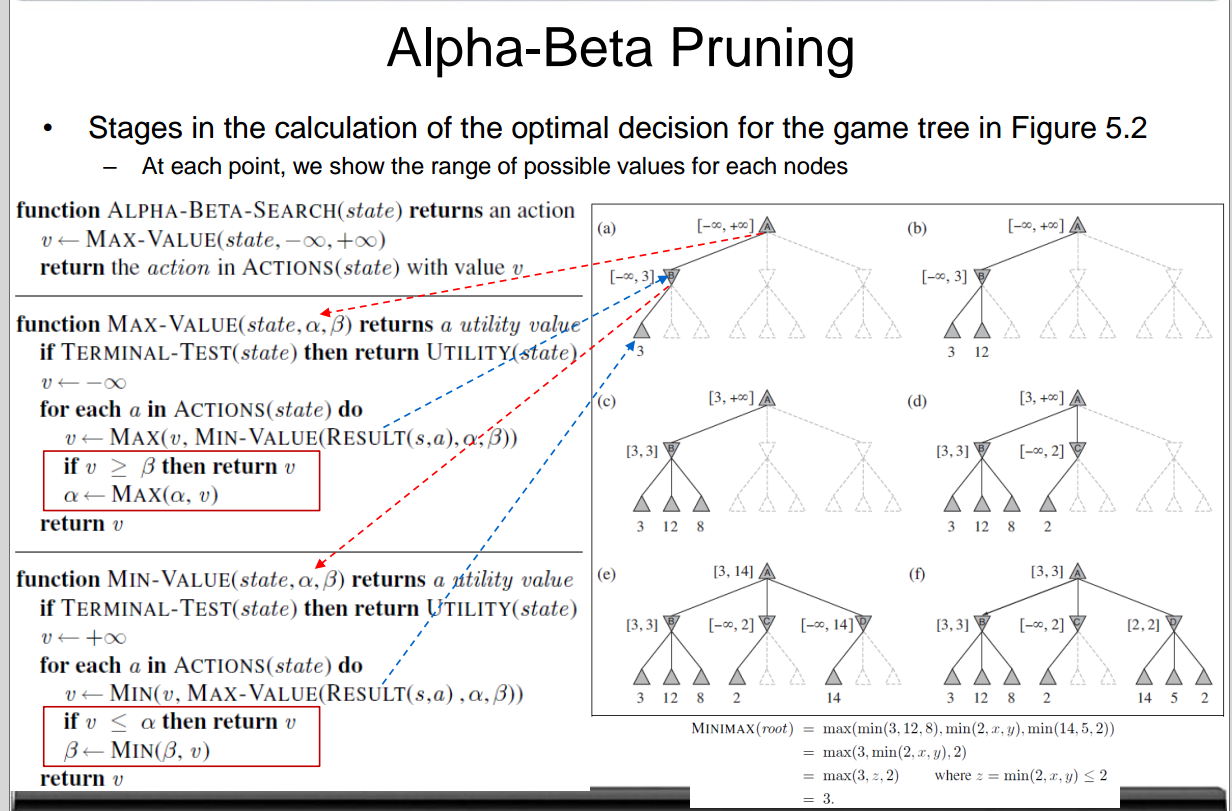
\includegraphics[width=0.9\textwidth]{ABP}
\subsection{Monte-Carlo Tree Search}
\label{sec:org3789fc4}

\section{Inference and Reasoning}
\label{sec:orgc7aa1b4}
\subsection{Propositional logic}
\label{sec:orgf2b54aa}
\subsection{Predicate logic}
\label{sec:orgc0cfbb2}
\subsection{First Order Inductive Learner}
\label{sec:org2cfddee}
\textbf{knowledge graph}: node = entity, edge = relation.
triplet (head entity, relation, tail entity)
\section{Statistical learning and modeling}
\label{sec:org9a7291c}
\subsection{Machine Learning: the concept}
\label{sec:org12226bf}
\subsubsection{Example and concept}
\label{sec:org08f7868}
\begin{description}
\item[{Supervised learning problems}] applications in which the \textbf{training data} comprises examples of the input
vectors along with their corresponding \textbf{target vectors} are known

classification and regression
\item[{Unsupervised learning problems}] the training data consists of a set of input vectors X \textbf{without any
corresponding target values}

density estimation, clustering, hidden markov models
\item[{Reinforcement learning problem}] finding suitable actions to take in a given situation in order to
maximize a reward. Here the learning algorithm is not given examples of
optimal outputs, in contrast to supervised learning, but must instead
discover them by a process of trial and error. A general feature of
reinforcement learning is the trade-off between exploration and exploitation
\end{description}

types of machine learning
\begin{itemize}
\item supervised learning
\begin{itemize}
\item classification: the output is categorical or nominal variable
\item regression: the output is read-valued variable
\end{itemize}
\item unsupervised learning
\item semi-supervised learning
\item reinforcement learning
\item deep learning
\end{itemize}
\subsubsection{supervised learning: important concepts}
\label{sec:org22da553}
\begin{itemize}
\item Data: labeled instances \(<\bl{x}_i,\bl{y}>\)
\item features: attribute-value pairs which characterize each \(\bl{x}\)
\item learning a discrete function: \textbf{classification}
\item learning a continuous function: \textbf{regression}
\end{itemize}

\textbf{Classification} - A two-step process
\begin{itemize}
\item \textbf{model construction}
\item \textbf{model usage}
\end{itemize}

\textbf{regression}
\begin{itemize}
\item Example: price of a used car

\(\bl{x}\): car attributes. \(\bl{y}=g(\bl{x}\mid\bl{\theta})\): price. \(g\):
model. \(\theta\) parameter set.
\end{itemize}
\subsection{example: polynomial curve fitting}
\label{sec:orgec139a3}
cross validation


SSE error(sum-of-square) \(E(\bl{w})=\frac{1}{2}\displaystyle\sum_{n=1}^N
   \lb y(x_n,\bl{w})-t_n\rb^2\)

RMS(root-mean-square) error \(E_{RMS}=\sqrt{2E(\bl{w}^*)/N}\)

high variance -> overfitting

How to control over-fitting
\begin{enumerate}
\item more train data
\item regularization
\item bayesian approach
\item cross-validation
\end{enumerate}


curse of dimensionality
\begin{itemize}
\item Extend polynomial curve fitting approach to deal with input spaces having
several variables. If we have D input variables, then a general polynomial
with coefficients up to order 3 would take the form:

\begin{equation*}
y(\bl{x},\bl{w})=w_0+\displaystyle\sum_{i=1}^Dw_ix_i+
\displaystyle\sum_{i=1}^D \displaystyle\sum_{j=1}^Dw_{ij}x_ix_j+
\displaystyle\sum_{i=1}^D \displaystyle\sum_{j=1}^D
\displaystyle\sum_{k=1}^Dw_{ijk}x_ix_jx_k
\end{equation*}
\end{itemize}
\subsection{probability theory review and notation}
\label{sec:org6674145}
rules of probability
\begin{itemize}
\item \textbf{sum rule} \(p(X)=\displaystyle\sum_Yp(X,Y)\)
\item \textbf{product rule} \(p(X,Y)=p(Y|X)p(X)\)
\end{itemize}

Bayes' Theorem: \(p(Y|X)=\frac{p(X|Y)p(Y)}{p(X)}\). Using sum rule
\(p(X)=\displaystyle\sum_Yp(X|Y)p(Y)\)

probability densities. 
\begin{align*}
p(x\in(a,b))&=\int_a^bp(x)dx\\
P(z)&=\int_{-\infty}^z p(x)dx\\
\int_{-\infty}^\infty p(x)dx&=1\quad p(x)\le0
\end{align*}
\(p(x)\) must satisfy two conditions
\begin{align*}
p(x)&\le 0\\
\int_{-\infty}^\infty p(x)dx&=1
\end{align*}


\textbf{expectation} \(\mathbb{E}[f]=
   \begin{cases}
   \displaystyle\sum_{x}p(x)f(x) & \text{discrete variables}\\
   \int p(x)f(x)dx & \text{continuous variables}
   \end{cases}\). In either cases,
\(\mathbb{E}[f]\approx\frac{1}{N}\displaystyle\sum_{n=1}^N f(x_n)\).
\textbf{conditional expectation}: \(\mathbb{E}_x[f| y]=\displaystyle\sum_xp(x| y)f(x)\).

The \textbf{variance} of \(f(x)\) is

\begin{align*}
var[f]&=\mathbb{E}[(f(x)-\mathbb{E}[f(x)])^2]\\
&=\mathbb{E}[f(x)^2-2f(x)\mathbb{E}[f(x)]+\mathbb{E}[f(x)]^2]\\
&=\mathbb{E}[f(x)^2]-\mathbb{E}[f(x)]^2
\end{align*}


The \textbf{covariance} is

\begin{align*}
cov[x,y]&=\mathbb{E}_{x,y}[(x-\mathbb{E}[x])(y-\mathbb{E}[y])]\\
&=\mathbb{E}_{x,y}[xy]-\mathbb{E}[x]\mathbb{E}[y]
\end{align*}


\begin{equation*}
\mathbb{V}[X]=\sigma^2_X=\E[(X-\E[X])^2]=\E[X^2]-\E[X]^2
\end{equation*}
\begin{equation*}
\V[\displaystyle\sum_{i=1}^nX_i]=\displaystyle\sum_{i=1}^n\V[X_i]+
\displaystyle\sum_{i\neq j}\text{Cov}[X_i,X_j]
\end{equation*}

\begin{align*}
&\text{Cov}[X,X]=\V[X]\\
&\text{Cov}[aX,bY]=ab\text{Cov}[X,Y]\\
&\text{Cov}[X+a,Y+b]=\text{Cov}[X,Y]
\end{align*}
\emph{the variance of the sum of two independent random variables is the sum of}
\emph{variance}. Given
\begin{center}
\begin{tabular}{c|c}
X & probability\\
\hline
\(x_1\) & \(p_1\)\\
\(\dots\) & \(\dots\)\\
\(x_n\) & \(p_n\)\\
\end{tabular}
\end{center}

\begin{center}
\begin{tabular}{c|c}
Y & probability\\
\hline
\(y_1\) & \(q_1\)\\
\(\dots\) & \(\dots\)\\
\(y_m\) & \(q_m\)\\
\end{tabular}
\end{center}
\begin{align*}
var(X+Y)=var(X)+var(Y)
\end{align*}

In case of two vectors of random variables \(\bl{x}\) and \(\bl{y}\), the
covariance is a matrix
\begin{align*}
cov[\bl{x},\bl{y}]&=\mathbb{E}_{\bl{x},\bl{y}}[(\bl{x}-\mathbb{E}[\bl{x}])(\bl{y}^T
-\mathbb{E}[\bl{y}^T])]\\
&=\mathbb{E}_{\bl{x},\bl{y}}[\bl{xy}^T]-\mathbb{E}[\bl{x}]\mathbb{E}[\bl{y}^T]
\end{align*}

\textbf{Bayesian probabilities}: \(P(A|B)=\frac{P(B|A)P(A)}{P(B)}\),
\(p(\mathcal{D})=\int p(\mathcal{D}|\bl{w})p(\bl{w})\text{d}\bl{w}\)
. For a data set 
\(\mathcal{D}=\{t_1,\dots,t_n\}\) and assumption \(w\),
\(p(w|\mathcal{D})=\frac{p(\mathcal{D}|w)p(w)}{p(\mathcal{D})}\). \(p(w)\) is
\textbf{prior probability}, \(p(\mathcal{D}|w)\) is \textbf{likelihood} (the probability
\(\mathcal{D}\) happens). Hence 
\begin{equation*}
\text{posterior}\propto\text{likelihood}\times\text{prior}
\end{equation*}

\textbf{Gaussian distribution}.
\begin{equation*}
\mathcal{N}(x|\mu,\sigma^2)=\frac{1}{(2\pi\sigma^2)^{1/2}}\exp\left\{
-\frac{1}{2\sigma^2}(x-\mu)^2\right\}
\end{equation*}
\(\mu\) is called \textbf{mean}, \(\sigma^2\) is called \textbf{variance}, \(\sigma\) \textbf{standard
deviation}, \(\beta=1/\sigma^2\) \textbf{precision}
\begin{align*}
\mathbb{E}[x]&=\int_{-\infty}^\infty\mathcal{N}(x|\mu,\sigma^2)xdx=\mu\\
\mathbb{E}[x^2]&=\int_{-\infty}^\infty\mathcal{N}(x|\mu,\sigma^2)x^2dx=\mu^2
+\sigma^2\\
var[x]&=\mathbb{E}[x^2]-\mathbb{E}[x]^2=\sigma^2\\
\end{align*}
For \$D\$-dimensional vector \(\bl{x}\) of continuous variables
\begin{equation*}
\mathcal{N}(\bl{x}|\bl{\mu},\bl{\Sigma})=\frac{1}{(2\pi)^{D/2}}\frac{1}
{\abs{\bl{\Sigma}}^{1/2}}\exp\left\{-\frac{1}{2}(\bl{x}-\bl{\mu})^T
\bl{\Sigma^{-1}}(\bl{x}-\bl{\mu})\right\}
\end{equation*}

To determine values for the unknown parameters given \(\mu\) and \(\sigma^2\) by
maximizing the likelihood function. Use log.
\begin{align*}
P(\bl{X}|\mu,\sigma^2)&=\displaystyle\prod_{n=1}^N\mathcal{N}(x_n|\mu,\sigma^2)\\
\Rightarrow \ln P(\bl{X}|\mu,\sigma^2)&=-\frac{1}{2\sigma^2}
\displaystyle\sum_{n=1}^N(x_n-\mu)^2-\frac{N}{2}\ln\sigma^2-\frac{N}{2}\ln(2\pi)\\
\end{align*}
Hence \(\mu_{ML}=\frac{1}{N}\displaystyle\sum_{n=1}^Nx_n\),
\(\sigma^2_{ML}=\frac{1}{N}\displaystyle\sum_{n=1}^N(x_n-\mu_{ML})^2\) by
partial derivative.
\(\E[\sigma_{ML}^2]=(\frac{N-1}{N})\sigma^2\)

Maximum likelihood estimator for mean is unbiased, that
  is, \(\mathbb{E}(\mu_{ML})=\mu\). Maximum likelihood estimator for variance is
  biased. \(\mathbb{E}(\sigma_{ML}^2)=\mathbb{E}(x^2)-\mathbb{E}(\mu_{ML}^2)=
   \frac{N-1}{N}\sigma_x^2\)



\subsection{information theory}
\label{sec:org881e2c9}
\textbf{entropy}: measuring uncertainty of a random variable \(X\).
\(H(X)=H(p)=-\displaystyle\sum_{x\in\Omega}p(x)\log p(x)\) where \(\Omega\) is
all possible values and define \(0\log0=0,\log=\log_2\)

\(H(X)=\displaystyle\sum_{x\in\Omega}p(x)\log_2\frac{1}{p(x)}=
   E(\log_2\frac{1}{p(x)})\). And "information of \(x\)"​="\#bits to code \(x\)"​=\(-\log
   p(x)\)

\textbf{Kullback-Leibler divergence}: comparing two distributions
\(D_{KL}(p||q)=H(p,q)-H(p)=-\int p(\bl{x})\ln\lb
   \frac{q(\bl{x})}{p(\bl{x})}\rb d\bl{x}\)

\url{https://www.youtube.com/watch?v=ErfnhcEV1O8}


\textbf{mutual information}
\(I[\bl{x},\bl{y}]=\text{KL}(p(\bl{x},\bl{y})||p(\bl{x})p(\bl{y}))=H(\bl{y})-H[\bl{y}|\bl{x}]\)
\subsection{The gaussian distribution}
\label{sec:org41f3e18}
\begin{align*}
\Delta^2&=(x-\mu)^T\Sigma^{-1}(x-\mu)\\
&=(x-\mu)^TU\Lambda^{-1}U^T(x-\mu)\\
&=(U^T(x-\mu))^T\Lambda^{-1}(U^T(x-\mu))=y^T\Lambda^{-1}y
\end{align*}


\(\Sigma u_i=\lambda_i u_i\) where \(i=i,\dots,D\).
\begin{equation*}
\Sigma U=\Sigma(u_1,\dots,u_D)=(u_1,\dots,u_D)
\begin{pmatrix}
\lambda_1 & \dots & 0\\
\vdots & \ddots & \vdots\\
0&\dots &\lambda_D
\end{pmatrix}=U\Lambda
\end{equation*}

\(\forall i,j\in\lb 1,\dots,D\rb\),
\begin{equation*}
u_i^Tu_j=I_{ij}=
\begin{cases}
1&\text{if } i=j\\
0%\text{otherwise}
\end{cases}
\end{equation*}

\begin{equation*}
U^TU=I
\end{equation*}
So \(U\) is orthogonal, \(\Sigma UU^T=U\Lambda
   U^T=\displaystyle\sum_{i=1}^D\lambda_i u_iu_i^T\), and \(\Sigma^T=U\Lambda^{-1}U^T\)

\begin{equation*}
\Delta^2=\bl{y}^T\Lambda^{-1}\bl{y}\xrightarrow{y_i=\bl{u}_i^T(\bl{x}-\bl{\mu})}
\displaystyle\sum_{i=1}^D\frac{y_i^2}{\lambda_i}
\end{equation*}


GIven a square matrix \(A\in\R^{n\times n},x\in\R^n\), \(x^TAx\) is called a
\textbf{quadratic form}
\begin{equation*}
x^TAx=\displaystyle\sum_{i=1}^nx_i(Ax)_i=\displaystyle\sum_{i=1}^n x_i
(\displaystyle\sum_{j=1}^nA_{ij}x_j)=\displaystyle\sum_{i=1}^n
\displaystyle\sum_{j=1}^nA_{ij}x_ix_j
\end{equation*}

\begin{equation*}
x^TAx=(x^TAx)^T=x^T(1/2A+1/2A^T)x
\end{equation*}

Let \(A=\Sigma^{-1}\), if A is not symmetric, let \(A^*=(A+A^T)/2\), then it's
symmetric

\begin{equation*}
\text{cov}[\bl{x}]=\E[\bl{xx}^T]-(\E[\bl{x}])^2=\bl{\mu\mu}^T-\bl{\Sigma}-\bl{\mu}^2=\bl{\Sigma}
\end{equation*}


   \begin{align*}
&p(\bX|\bmu,\bSigma)=\displaystyle\prod_{n=1}^N\caln(\bx_n|\bmu,\bSigma)\\
&\ln p(\bl{X}|\bl{\mu}, \bl{\Sigma})=-\frac{ND}{2}\ln(2\pi)-\frac{N}{2}\ln\abs{\bSigma}
-\frac{1}{2}\displaystyle\sum_{n=1}^N(\bx_n-\bmu)^T\bSigma^{-1}(\bx_n-\bmu)\\
&\frac{\partial}{\partial\bSigma}\ln p(\bX|\bmu,\bSigma)=
-\frac{N}{2}\frac{\partial}{\partial\bSigma}\lb\abs{\bSigma}-\frac{\partial}{2\partial\bSigma}
\displaystyle\sum_{n=1}^N(\bx_n-\bmu)^T\bSigma^{-1}(\bx_n-\bmu)\rb\\
&\text{Since } \frac{\partial\ba^T\bX^{-1}\bb}{\partial\bX}=-\bX^{-1}\ba\bb^T\bX^{-1},\quad
\frac{\partial}{\partial \bA}\ln\abs{\bA}=(\bA^{-1})^T\\
&-\frac{N}{2}\bSigma^{-1}+\frac{N}{2}\bSigma^{-1}\bS\bSigma^{-1}=0,\quad
\bS=\frac{1}{N}\displaystyle\sum_{n=1}^N(\bx_n-\bmu)(\bx_n-\bmu)^T\\
&\bSigma=\bS=\bSigma_{ML}
\end{align*}


\begin{align*}
\E[\bSigma_{ML}]&=\frac{1}{N}\displaystyle\sum_{n=1}^N\E[\lb(\bx_n-\frac{1}{N}
\displaystyle\sum_{m=1}^N\bx_m)(\bx_n^T-\frac{1}{N}\displaystyle\sum_{l=1}^N\bx_l^T)]\rb\\
&=\frac{1}{N}\displaystyle\sum_{n=1}^N\E[\bx_n\bx_n^T-\frac{2}{N}\bx_n
\displaystyle\sum_{m=1}^N\bx_m^T+\frac{1}{N^2}
\displaystyle\sum_{m=1}^N \displaystyle\sum_{l=1}^N\bx_m\bx_l^T]\\
&=\bmu\bmu^T+\bSigma-2(\bmu\bmu^T+\frac{1}{N}\bSigma)+\bmu\bmu^T+\frac{1}{N}\bSigma\\
&=(\frac{N-1}{N})\bSigma
\end{align*}
\subsection{Nonparametric methods}
\label{sec:orge6c6a30}
How to estimate unknown probability densituy \(p(x)\):
\begin{itemize}
\item Assume we have collected a data set comprising N observations drawn from
p(x). Consider some small region R containing x, the probability mass
associated with this region is given by
\begin{equation*}
P=\int_\mathcal{R}p(\bx)d\bx\quad\Rightarrow\quad p(\bx)=\frac{K}{NV}
\end{equation*}
\item V is the volumn of R
\item K is the total number of points that lie inside R
\end{itemize}


\begin{enumerate}
\item \textbf{Kernel density estimator}

Fix V, determine K from the data
\item \textbf{KNN density estimator}

Fix K, determine the value of V from the data
\end{enumerate}
\subsubsection{Kernel density estimators}
\label{sec:org5060c3d}
Parzen window
\begin{equation*}
k(\bu)=
\begin{cases}
1&\abs{u_i}\le 1/2,i=1,\dots,D\\
0&\text{otherwise}
\end{cases}
\end{equation*}
\begin{itemize}
\item The total number of data points lying inside this cube:
\begin{equation*}
K=\displaystyle\sum_{n=1}^N k(\frac{\bx-\bx_n}{h})
\end{equation*}
\item The estimated density at x:
\begin{equation*}
p(\bx)=\frac{1}{N}\displaystyle\sum_{n=1}^N\frac{1}{h^D}k(\bx-\bx_n){h}
\end{equation*}
\end{itemize}
\subsubsection{Nearest-neighbour methods}
\label{sec:orgb212ee1}
Fix K, determine the value of V from the data


KNN classifier
\begin{align*}
&p(\bx|\calc_k)=\frac{K_k}{N_kV}\\
&p(\calc_k)=\frac{N_k}{N}\\
&p(\calc_k|\bx)=\frac{p(\bx|\calc_k)p(\calc_k)}{p(\bx)}=\frac{K_k}{K}\\
&p(\bx)=\frac{K}{NV}
\end{align*}


\begin{itemize}
\item \textbf{training phase}

storing the d-Dim feature vectors and class labels of the training samples
\item \textbf{testing phase}

 An object is classified by a majority vote of its neighbors, with the
object being assigned to the class most common among its k nearest
neighbors (k = 1,3,5,…)
\end{itemize}
\subsection{Linear model for classification}
\label{sec:org2eecf12}
\textbf{Regression}: given a training data set comprising \(N\) observations
\(\lb\bx_n\rb\), where \(n=1,\dots,N\) together with corresponding target values
\(\lb t_n\rb\), the goal is to predict the value of \(t\) for a new value of
\(\bx\)

\textbf{linear regression}: \(y(\bl{x},\bl{w})=w_0+w_1x_1+\dots+w_Dx_D=\bl{w}^T\bl{x}\)
where \(\bx=(x_1,\dots,x_D)^T\)


\textbf{linear basis function model}: Linear combinations of fixed nonlinear functions
of the input variables 
\begin{equation*}
y(\bl{x},\bl{w})=w_0+\displaystyle\sum_{j=1}^{M-1}w_j\phi_j(\bl{x})
=\bl{w}^T\bl{\phi(\bl{x})} 
\end{equation*}
where \(\phi_0(\bx)=1\), \(\bphi=(\phi_0,\dots,\phi_{M-1})^T\), 
\(\bw=(w_0,\dots,w_{M-1})\)


\begin{enumerate}
\item polynomial basis function \(\phi_j(x)=x^j\)
\item Gaussian basis function: \(\phi_j(x)=\exp\lb-\frac{(x-\mu_j)^2}{2s^2}\rb\)
\item sigmoid basis function: \(\phi_j(x)=\sigma(\frac{x-\mu_j}{s})\),
\(\sigma(a)=\frac{1}{1+\exp(-a)}\)
\end{enumerate}
\subsubsection{Maximum likelihood and least squares}
\label{sec:orge6bd462}
Assume target variable \(t\) is given by a deterministic function
\(y(\bl{x},\bl{w})\) with additive Gaussian noice so that
\(t=y(\bl{x},\bl{w})+\epsilon\) where \(\epsilon\) is a zero mean Gaussian
random variable with precision \(\beta\), hence we can write
\begin{equation*}
p(t|\bl{x},\bl{w},\beta)=\mathcal{N}(t|y(\bl{x},\bl{w}),\beta^{-1})
\end{equation*}
and \(\mathbb{E}(t|\bl{x})=\int tp(t|\bl{x})dt=y(\bl{x},\bl{w})\)


For data set \(\bl{X}=\{\bl{x}_1,\dots,\bl{x}_n\},\bl{t}=(t_1,\dots,t_n)^T\),
\(p(\bl{t}|\bl{X},\bl{w},\beta)=\displaystyle\prod_{n=1}^N\mathcal{N}(t_n|
    \bl{w}^T\bl{\phi}(\bl{x}_n),\beta^{-1})\)

\(\ln p(\bl{t}|\bl{w},\beta)=\displaystyle\sum_{n=1}^N\ln\mathcal{N}(t_n|
    \bl{w}^T\bl{\phi}(\bl{x}_n),\beta^{-1})=\frac{N}{2}\ln\beta-\frac{N}{2}\ln(2\pi)-
    \beta \boxed{E_D(\bl{w})}\)

\(E_D(\bl{w})=\frac{1}{2}\displaystyle\sum_{n=1}^N
    \left\{t_n-\bl{w}^T\bl{\phi}(\bl{x}_n)\right\}^2=
    \frac{1}{2}\norm{\bt -\Phi\bl{w}}\) is sum-of-squares error function

solve \(\bl{w}\) by maximum likelihood.
\begin{equation*}
\nabla\ln p(\bl{t}|\bl{w},\beta)=\displaystyle\sum_{n=1}^N
\left\{t_n-\bl{w}^T\bl{\phi}(\bl{x}_n)\right\}\phi(\bl{x}_n)^T
\end{equation*}
\begin{equation*}
0=\displaystyle\sum_{n=1}^N t_n\bl{\phi}(\bl{x}_n)^T-\bl{w}^T
(\displaystyle\sum_{n=1}^N\bl{\phi}(\bl{x}_n)\bl{\phi}(\bl{x}_n)^T)
\end{equation*}
Hence we get
\begin{equation*}
\bl{w}_{ML}=(\bl{\Phi}^T\bl{\Phi})^{-1}\bl{\Phi}^T\bl{t}
\end{equation*}
\(\Phi\) is \textbf{design matrix}.
\[
\Phi=\begin{pmatrix}
 \phi_0(\bl{x}_1) & \phi_1(\bl{x}_1) & \dots & \phi_{M-1}(\bl{x}_1) \\
 \phi_0(\bl{x}_2) & \phi_1(\bl{x}_2) & \dots & \phi_{M-1}(\bl{x}_2) \\
 \vdots & \vdots & \ddots & \vdots \\
 \phi_0(\bl{x}_N) & \phi_1(\bl{x}_N) & \dots & \phi_{M-1}(\bl{x}_N) \\
\end{pmatrix}
\]
For bias parameter \(w_0\).
\(E_D(\bl{w})=\frac{1}{2}\displaystyle\sum_{n=1}^N 
    \{t_n-w_0-\displaystyle\sum_{j=1}^{M-1}w_j\phi_j(\bl{x}_n)\}^2\). Hence
\(w_0=\bar{t}-\displaystyle\sum_{j=1}^{M-1}w_j\bar{\phi_j}\),
\(\bar{t}=\frac{1}{N}\displaystyle\sum_{n=1}^Nt_n\),
\(\bar{\phi_j}=\frac{1}{N}\displaystyle\sum_{n=1}^N\phi_j(\bl{x}_n)\).

Solving the noise precision parameter \(\beta\) by ML
\(\frac{N}{2\beta}=E_D(\bl{w})\). \(\frac{1}{\beta_{ML}}=
    \frac{1}{N}\displaystyle\sum_{n=1}^N\left\{t_n-\bl{w}^T_{ML}
    \bl{\phi}(\bl{x}_n)\right\}^2\)
\subsubsection{sequential learning}
\label{sec:org30bbdab}
\textbf{Gradient descent}: Gradient descent is based on the observation that if the
multivariable function \(J(\bw)\) is defined and differentiable in a neighborhood of a
point \(\bw_0\), then \(J(\bw)\) decreases \textbf{fastest} if one goes from \(\bw_0\) in the direction of
the negative gradient of J(.) at \(\bw_0-J'(\bw_0)\)
\begin{center}
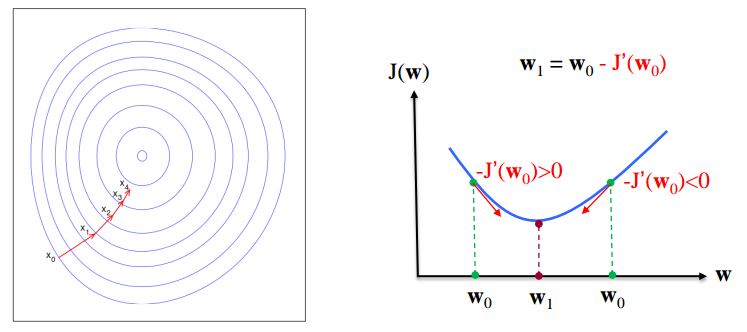
\includegraphics[width=0.8\textwidth]{GradientDescent}
\end{center}


batch gradient descent
\begin{align*}
&\bw^{(\tau+1)}=\bw^{(\tau)}-\eta\nabla E_D(\bw)\\
&E_D(\bw)=\frac{1}{2}\displaystyle\sum_{n=1}^N\lb t_n-\bw^T\bphi(\bx_n)\rb^2
=\frac{1}{2}\norm{\bt-\bPhi\bw}^2\\
&\bw^{(\tau+1)}=\bw^{(\tau)}+\eta\bPhi^T(\bt-\bPhi\bw^{(\tau)})
\end{align*}
if \(\bw^{(\tau+1)}=\bw^{(\tau)}\), then
\(\bw^{(\tau)}=(\bPhi^T\bPhi)^{-1}\bPhi^T\bt\)


stochastic gradient descent
\begin{equation*}
\bw^{(\tau+1)}=\bw^{(\tau)}-\eta\nabla E_n
\end{equation*}
\subsubsection{Regularized least squares}
\label{sec:org362b793}
Error function with regularization term
\begin{equation*}
E_D(\bw)+\lambda E_W(\bw)=\frac{1}{2}\norm{\bt-\bPhi\bw}+
\frac{\lambda}{2}\bw^T\bw
\end{equation*}

\begin{equation*}
\bw=(\lambda \bI+\bPhi^T\bPhi)^{-1}\bPhi^T\bt
\end{equation*}
\subsubsection{multiple outputs}
\label{sec:org85fe542}
\(\by(\bx,\bw)=\bW^T\bphi(\bx)\), \(\bW=(\bw_1,\dots,\bw_K)_{M\times K}\)

\(\bW_{ML}=(\bPhi^T\bPhi)^{-1}\bPhi^T\bT\)
\subsection{model selection}
\label{sec:orgc86465e}
\textbf{cross-validation}
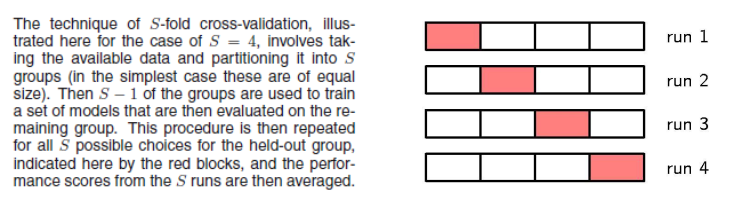
\includegraphics[width=100mm]{CrossValidation}

split training data into \textbf{training set} and \textbf{validation set}. Train different
models on training set and choose model with minimum error on validation set.
\subsection{decision theory}
\label{sec:org7aef8ed}
Suppose we have an input vector \(\bl{x}\) together with a corresponding vector
\(\bl{t}\) of target variables and our goal is to predict \(\bl{t}\) given new
value for \(\bl{x}\). The joint probability distribution \(p(\bl{x},\bl{t})\)
provides a complete summary of the uncertainty with these variables


misclassification rate
\begin{align*}
p(\text{mistake})&=p(\bx\in\calr_1,\calc_2)+p(\bx\in\calr_2,\calc_1)\\
&=\int_{\calr_1}p(\bx,\calc_2)d\bx+\int_{\calc_2}p(\bx,\calc_1)d\bx
\end{align*}

msupose loss matrix \(L\)

average loss \(\E[L]=\displaystyle\sum_k \displaystyle\sum_j
   \int_{\calr_j}L_{kj}p(\bx,\calc_k)d\bx\)

\begin{center}
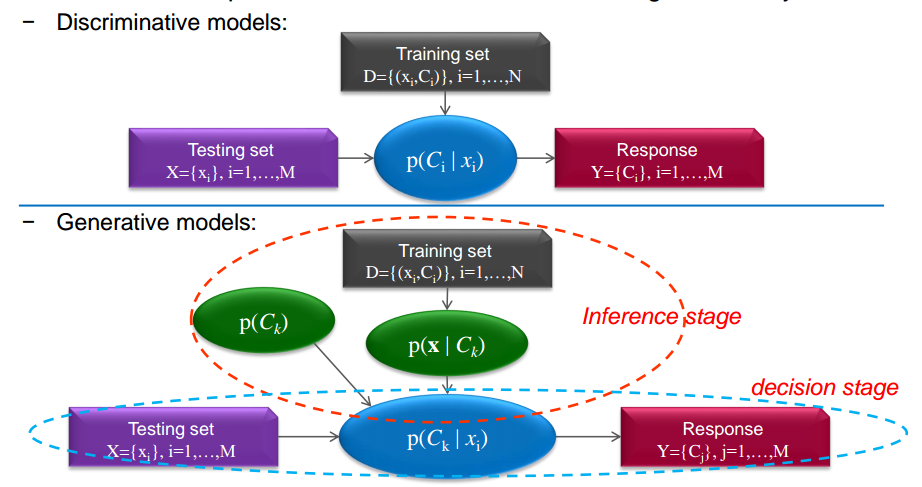
\includegraphics[width=.9\textwidth]{DecisionTheory}
\end{center}
\section{Statistical learning and modeling - Supervised learning}
\label{sec:org7020f24}
\subsection{Basic concepts}
\label{sec:org0a39595}
\begin{itemize}
\item \textbf{Linearly separable}
\begin{itemize}
\item decision regions:

input space is divided into several regions
\item decision boundaries:
\begin{itemize}
\item under linear models, it's a linear function
\item (D-1)-dimensional hyper-plane within the D-dimensional input space
\end{itemize}
\end{itemize}
\item \textbf{representation of class labels}
\begin{itemize}
\item Two classes K = 2
\item K classes
\begin{itemize}
\item 1-of-K coding scheme \(\bl{t}=(0,0,1,0,0)^T\)
\end{itemize}
\item Predict discrete class labels
\begin{itemize}
\item linear model prediction \(y(\bl{x})=\bl{w}^T\bl{x}+w_0\)

w: weight vector, w\textsubscript{0} bias/threshold

\item nonlinear function \(f(.):R\to(0,1)\)
\item generalized linear models

\(y(\bl{x})=f(\bl{w}^T\bl{x}+w_0)\)

f:activation function
\item dicision surface

\(y(\bl{x})=\text{constant}\to \bl{w}^T\bl{x}+w_0=\text{constant}\)
\end{itemize}
\end{itemize}
\item \textbf{Three classification approaches}
\begin{itemize}
\item discriminant function
\begin{itemize}
\item least squares approach
\item fisher's linear discriminant
\item the perceptron algorithm of rosenblatt
\end{itemize}
\item use discriminant functions directly and don't compute probabilities

Given discriminant functions \(f_1(\bl{x}),\dots,f_K(\bl{x})\). Classify
\(\bl{x}\) as class \(\mathcal{C}_k\) iff \(f_k(\bl{x})>f_j(\bl{x}),\forall
       j\neq k\)

\begin{itemize}
\item \textbf{least-squares approach}: making the model predictions as close as
possible to a set of target values
\item \textbf{fisher's linear discriminant}: maximum class separation in the ouput
space
\item \textbf{the perceptron algorithm of rosenblatt}
\end{itemize}
\item generative approach
\begin{itemize}
\item model the class-conditional densities and the class priors
\item compute posterior probabilities through Bayes's theorem

\(\underbrace{p(\mathcal{C}_k|\bl{x})}_\text{posterior for class}=
         \frac{\overbrace{p(\bl{x}|\mathcal{C}_k)}^\text{class conditional density}
         \overbrace{p(\mathcal{C}_k)}^\text{class prior}}{p(\bl{x})}=
         \frac{p(\bl{x}|\mathcal{C}_k)p(\mathcal{C}_k)}{\sum_{j}p(\bl{x}|\mathcal{C}_j)
         p(\mathcal{C}_j)}\)
\end{itemize}
\end{itemize}
\end{itemize}
\subsection{discriminant functions}
\label{sec:org484d9fd}
linear classification \(\by=y(\bx)=W^T\bx+\bw_0\)

Hinge loss(\(c\) is the true label)
\begin{equation*}
L_i=\displaystyle\sum_{j\in\lb 1,\dots,C\rb,j\neq c}
\max(0,y_i^j-y_i^c+\epsilon)
\end{equation*}

loss function with regularization
\(L=\frac{1}{N}\displaystyle\sum_{i=1,\dots,N}L_i+\alpha\varnothing(W)\)

dimensionality reduction
\begin{enumerate}
\item PCA - principal component analysis
\item SVD - singular value decomposition
\end{enumerate}
\subsubsection{Two classes}
\label{sec:org658fc71}
\begin{itemize}
\item Linear discriminant function \(y(\bl{x})=\bl{w}^T\bl{x}+w_0\)
\begin{itemize}
\item Dicision surface \(\Omega:y(\bl{x})=0\)
\item the normal distant from the origin to the dicision surface
\(\frac{\bl{w}^T\bl{x}}{\norm{\bl{w}}}=-\frac{w_0}{\norm{\bl{w}}}\)
\item if \(x_A,x_B\) lie on the decision surface \(y(\bl{x}_A)=y(\bl{x}_B)=0\),
then \(\bl{w}^T(\bl{x}_A-\bl{x}_B)=0\). hence w is orthogonal to every
vector lying within Ω. \(\frac{\bl{w}}{\norm{\bl{w}}}\) is the normal
vector of Ω

\item \(\bl{x}=\bl{x}_\perp+r\frac{\bl{w}}{\norm{\bl{w}}}\) hence
\(r=\frac{y(\bl{x})}{\norm{\bl{w}}}\). \(y(\bl{x}_\perp)=0\to
        \bl{w}^T\bl{x}=-w_0+r\frac{\bl{w}^T\bl{w}}{\norm{\bl{w}}}\)
\item \(\tilde{\bl{w}}=(w_0,\bl{w}), \tilde{\bl{x}}=(x_0,\bl{x}),
        y(\bl{x})=\tilde{\bl{w}}^T\tilde{\bl{x}}\)
\end{itemize}
\end{itemize}
\subsubsection{K-class}
\label{sec:org4316d7f}
\begin{itemize}
\item One-versus-the-rest classifier
K - 1 classifiers each of which solves a two-class problem
\item One-versus-one classifier
K(K-1)/2 binary discriminant functions
\item K-class discriminant classifier
\end{itemize}


\begin{center}
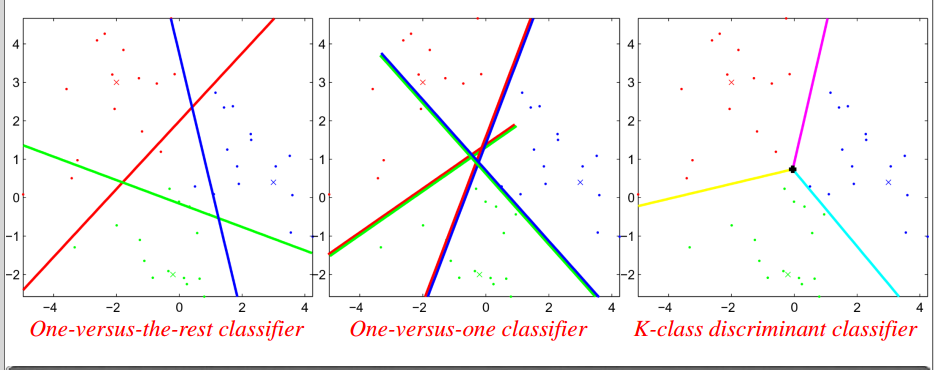
\includegraphics[width=.8\textwidth]{MultipleClasses}
\end{center}
\begin{itemize}
\item single K-class discriminant comprising K linear functions
\(y_k(\bl{x})=\bl{w}_k^T\bl{x}+w_{k_0}\)
\begin{itemize}
\item assigning a point x to class \(\mathcal{C}_k\) if
\(y_k(\bl{x}>y_j(\bl{x}))\) for all \(j\neq k\)
\item dicision boundary between class \(\mathcal{C}_k, \mathcal{C}_j\) is given
\(y_k(\bl{x})=y_j(\bl{x})\to
        (\bl{w}_k-\bl{w}_j)^T\bl{x}+(w_{k_0}-w_{j_0})=0\)
\item \(\mathcal{R}_k\) is singly connected convex
\item \(\hat{\bl{x}}=\lambda\bl{x}_A+(1-\lambda)\bl{x}_B\) where \(0\le\lambda\le
        1\), \(y_k(\hat{\bl{x}})=\lambda y_k(\bl{x}_A)+(1-\lambda)y_k(\bl{x}_B)\)
and hence \(\hat{x}\) also lies inside \(\mathcal{R}_k\)
\end{itemize}
\end{itemize}
\subsubsection{Learning the parameters of linear discriminant functions}
\label{sec:orgb7783a7}
\begin{enumerate}
\item Least-squares approach
\label{sec:org38e409d}
\begin{itemize}
\item Problem
\begin{itemize}
\item Each class \(\mathcal{C}_k\) is described by its own linear model 
\(y_k(\bl{x})=\bl{w}_k^T\bl{x}+w_{k0}\)
\item group together: \(y(\bl{x})=\widetilde{\bl{W}}^T\tilde{\bl{x}}\),
\(\tilde{\bl{w}}_k=(w_{k0},\bl{w}_k^T)^T\), \(\tilde{\bl{x}}=(1,\bl{x}^T)^T\)
\end{itemize}
\item Learning \(\widetilde{\bW}\) with training set \(\lb \bx_n,\bt_n\rb\)
\begin{itemize}
\item minimizing SSE function sum-of-squares
\(SSE=\displaystyle\sum_{i=1}^n(y_i-f(x_i))^2\)

\(E_D(\widetilde{\bl{W}})=1/2\text{Tr}\{(\bl{\widetilde{X}\widetilde{W}-T})^T 
         (\bl{\widetilde{X}\widetilde{W}-T})\}\)

\(\bl{\widetilde{W}}=(\bl{\widetilde{X}}^T\bl{\widetilde{X}})^{-1}\bl{\widetilde{X}}^T\bl{T}\)
\end{itemize}
\end{itemize}
\item fisher's linear discriminant
\label{sec:orgfda985a}

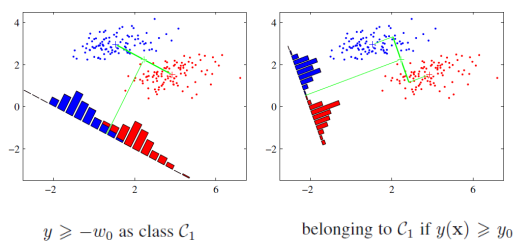
\includegraphics[width=100mm]{Fisher}

from the view of dimensionality reduction
\(y\ge -w_0\) as class \(\mathcal{C}_1\)

\(m_1=\frac{1}{N_1}\displaystyle\sum_{n\in\mathcal{C}_1}\bx_n, 
     m_2=\frac{1}{N_2}\displaystyle\sum_{n\in\mathcal{C}_2}\bx_n
     \xrightarrow{y=\bl{w}^T\bl{x}} m_2-m_1=\bl{w}^T(\bl{m}_2-\bl{m}_1)\)

\textbf{Fisher's criterion}: maximize the separation between the projected class
means as well as the inverse of the total within-class variance.

within-class variance \(s_k^2=\displaystyle\sum_{n\in\calc_k}(y_n-m_k)^2\),
\(y=\bw^T\bx,m_k=\bw^T\bm_k\)


generalized rayleigh quotient
\begin{equation*}
J(\bw)=\frac{(m_2-m_1)^2}{s_1^2+s_2^2}=\frac{\bw^T\bS_B\bw}{\bw^T\bS_W\bw}
\end{equation*}

between-class covariance matrix \(\bS_B=(\bm_2-\bm_1)(\bm_2-\bm_1)^T\)

within-class covariance matrix \(\bS_W=\displaystyle\sum_{n\in\calc_1}
     (\bx_n-\bm_1)(\bx_n-\bm_1)^T+
     \displaystyle\sum_{n\in\calc_2}(\bx_n-\bm_2)(\bx_n-\bm_2)^T\)


\textbf{Fisher's linear discriminant}:
\(\nabla J(\bw)=0\Rightarrow(\bw^T\bS_B\bw)\bS_W\bw=(\bw^T\bS_w\bw)\bS_B\bw\)

hence
\begin{equation*}
\bw\;\propto\;\bS_W^{-1}(\bm_2-\bm_1)
\end{equation*}
\item the perceptron algorithm of rosenblatt
\label{sec:org9377835}

construct a generalized linear model
\begin{equation*}
y(\bx)=f(\bw^T\bphi(\bx))\quad f(a)=
\begin{cases}
+1&a\ge 0\\
-1&a<0
\end{cases}
\end{equation*}


\(\bphi_n=\bphi(\bx_n)\)

perceptron criterion(minimize):
\(E_P(\bw)=-\displaystyle\sum_{n\in\calm}\bw^T\bphi_n t_n\), \(t\in\lb
     +1,-1\rb\)


\begin{equation*}
\bw^{(\tau+1)}=\bw^{(\tau)}-\eta\nabla E_P(\bw)=\bw^{(\tau)}+\eta\bphi_nt_n
\end{equation*}


Perceptron convergence theorem: If there exists an exact solution (in other
words, if the training data set is linearly separable), then the perceptron
learning algorithm is guaranteed to find an exact solution in a finite
number of steps
\end{enumerate}
\subsection{probalibilistic generative models}
\label{sec:orgd014300}
Determine the class conditional densities and class-specifix priors, and then
use Bayes' rule to obtain the posterior probabilites

A probabilistic view of classification from simple assumptions about the
distribution of the data

\begin{align*}
p(\mathcal{C}_1|\bl{x})&=\frac{p(\bl{x}|\mathcal{C}_1)p(\mathcal{C}_1)}
{p(\bl{x}|\mathcal{C}_1)p(\mathcal{C}_1)+p(\bl{x}|\mathcal{C}_2)p(\mathcal{C}_2)}\\
&=\frac{1}{1+\exp(-a)}=\sigma(a)
\end{align*}
where 
\begin{equation*}
a=\ln\frac{p(\bl{x}|\mathcal{C}_1)p(\mathcal{C}_1)}
{p(\bl{x}|\mathcal{C}_2)p(\mathcal{C}_2)}
\end{equation*}
and \(\sigma(a)\) is the \textbf{logistic sigmoid} function defined by
\begin{equation*}
\sigma(a)=\frac{1}{1+\exp(-a)}
\end{equation*}
and \(\sigma(-a)=1-\sigma(a)\), its inverse is \textbf{logit} function
\begin{equation*}
a=\ln(\frac{\sigma}{1-\sigma})
\end{equation*}

For case of \(K > 2\) classes, we have the following \textbf{multi-class generalization}
\begin{equation*}
p(\mathcal{C}_k|\bl{x})=\frac{p(\bl{x}|\mathcal{C}_k)p(\mathcal{C}_k)}
{\sum_jp(\bl{x}|\mathcal{C}_j)p(\mathcal{C}_j)}=\frac{\exp(a_k)}{\sum_j\exp(a_j)},
a_k=\ln\left[p(\bl{x}|\mathcal{C}_k)p(\mathcal{C}_k)\right]
\end{equation*}
The \textbf{normalized exponential} is known as the \textbf{softmax function} as it represents
a \emph{smoothed version of the max function}
\begin{equation*}
\text{if } a_k\ll a_j,\forall j\neq k,\text{then } p(\mathcal{C}_k|\bl{x})\approx 1,
p(\mathcal{C}_j|\bl{x})\approx 0
\end{equation*}

For \textbf{continuous inputs}, assume
\begin{equation*}
p(\bl{x}|\mathcal{C}_k)=\frac{1}{(2\pi)^{D/2}}\frac{1}
{\abs{\bl{\Sigma}}^{1/2}}\exp\left\{-\frac{1}{2}(\bl{x}-\bl{\mu}_k)^T
\bl{\Sigma^{-1}}(\bl{x}-\bl{\mu}_k)\right\}
\end{equation*}
\begin{enumerate}
\item 2 classes
\begin{align*}
p(\mathcal{C}_1|\bl{x})&=\sigma(\bl{w}^T\bl{x}+w_0)\\
\bl{w}&=\bl{\Sigma}^{-1}(\bl{\mu}_1-\bl{\mu}_2)\\
w_0&=-\frac{1}{2}\bl{\mu}_1^T\bl{\Sigma}^{-1}\bl{\mu}_1+
\frac{1}{2}\bl{\mu}_2^T\bl{\Sigma}^{-1}\bl{\mu}_2+\ln\frac{p(\mathcal{C}_1)}
{p(\mathcal{C}_2)}\\
\end{align*}
\item K classes
\begin{align*}
a_k(\bl{x})&=\bl{w}_k^T\bl{x}+w_{k0}\\
\bl{w}_k&=\bl{\Sigma}^{-1}\bl{\mu}_k\\
w_{k0}&=-\frac{1}{2}\bl{\mu}_k^T\bl{\Sigma}^{-1}\bl{\mu}_k+\ln p(\mathcal{C}_k)
\end{align*}
\end{enumerate}


Maximum likelihood solution for two classes. Assume 
\(p(\bx_n|\calc_n)=\caln(\bx_n|\bmu_k,\bSigma)\) and \(p(\calc_1)=\pi,
   p(\calc_2)=1-\pi\). We have \(\lb x_n,t_n\rb\) where \(t_n=1\) denotes class
\(\calc_1\)

\begin{equation*}
p(\bt|\pi,\bmu_1,\bmu_2,\bSigma)=\displaystyle\prod_{n=1}^N
[\pi\caln(\bx_n|\bmu_1,\bSigma)]^{t_n}[(1-\pi)\caln(\bx_n|\bmu_2,\bSigma)]^{1-t_n}
\end{equation*}

\begin{equation*}
 \ln p(\bt|\pi,\bmu_1,\bmu_2,\bSigma)=\displaystyle\sum_{n=1}^N\lb
 t_n\ln \pi+(1-t_n)\ln(1-\pi)+t_n\ln\caln(\bx_n|\bmu_1,\bSigma)+
 (1-t_n)\ln\caln(\bx_n|\bmu_2,\bSigma)
 \rb
\end{equation*}

\begin{enumerate}
\item solve \(\pi\)

\(\pi=\frac{N_1}{N_1+N_2}\)
\item solve \(\bmu_1,\bmu_2\)

\begin{equation*}
\displaystyle\sum_{n=1}^Nt_n\ln\caln(\bx_n|\bmu_1,\bSigma)=-\frac{1}{2}
\displaystyle\sum_{n=1}^Nt_n(\bx_n-\bmu_1)^T\bSigma^{-1}(\bx_n-\bmu_1)+\text{const}
\end{equation*}

\(\bmu_1=\frac{1}{N_1}\displaystyle\sum_{n=1}^Nt_n\bx_n,
      \bmu_2=\frac{1}{N_2}\displaystyle\sum_{n=1}^N(1-t_n)\bx_n\)
\item solve \(\bSigma\)

\begin{equation*}
\bS=\frac{N_1}{N}\boxed{\frac{1}{N_1}\displaystyle\sum_{n\in\calc_1}(\bx_n-\bmu_1)
(\bx_n-\bmu_1)^T}_{S_1}+\frac{N_2}{N}
\boxed{\frac{1}{N_2}\displaystyle\sum_{n\in\calc_2}(\bx_n-\bmu_2)(\bx_n-\bmu_2)^T}_{S_2}x
\end{equation*}

\(\bSigma_{ML}=\bS\)
\end{enumerate}
\subsection{probabilistic discriminative models}
\label{sec:orga4b2fcd}
train all of the model parameters to maximize the probability of getting the
label right. Model \(p(\calc_k|\bx)\) directly


\textbf{logistic sigmoid function}
\begin{equation*}
p(\calc_1|\bx)=\frac{1}{1+\exp(-\bw^T\bx)}=\sigma(\bw^T\bx)
\end{equation*}
training dataset \(\lb \bx_n,t_n\rb\), \(t_n\in\lb 0,1\rb\)

maximize the probability of getting the label right, so
\begin{equation*}
p(\bt|\bX,\bw)=\displaystyle\prod_{n=1}^N\left[y_n^{t_n}(1-y_n)^{1-t_n}\right],\quad
y_n=\sigma(\bw^T\bx_n)
\end{equation*}

\textbf{cross-entropy error function}
\begin{equation*}
E(\bw)=-\ln p(\bt|\bX,\bw)=-\displaystyle\sum_{n=1}^N\left[
t_n\ln y_n+(1-t_n)\ln(1-y_n)\right]=\displaystyle\sum_{n=1}^N E_n=
\displaystyle\sum_{n=1}^N H(p,q)
\end{equation*}

hence
\begin{equation*}
\nabla E(\bw)=\displaystyle\sum_{n=1}^N(y_n-t_n)\bx_n
\end{equation*}
the same form as the gradient of the sum-of-squares error function


\textbf{logistic regression model}: \(p(\calc_1|\phi)=y(\phi)=\sigma(\bw^T\bphi)\).
Only \textbf{M} parameters need to be estimated

\begin{equation*}
\nabla E(\bw)=\displaystyle\sum_{n=1}^N(y_n-t_n)\phi_n
\end{equation*}


\emph{Newton-raphson} iterative optmization scheme
\begin{equation*}
\bw^{\text{new}}=\bw^{\text{old}}-\bH^{-1}\nabla E(\bw)
\end{equation*}
\subsection{Boosting}
\label{sec:org880decd}
Originally designed for classification problems.

Motivation: a procedure that combines the outputs of many "weak" classifiers
to produce a strong/accurate classifier

\begin{center}
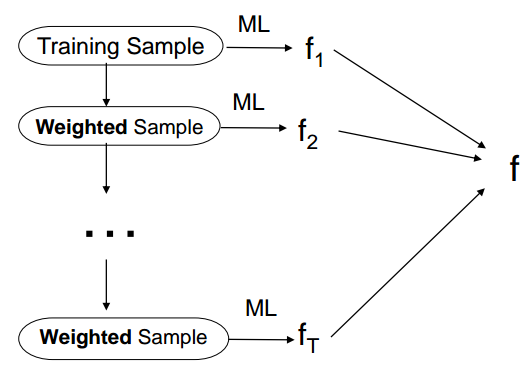
\includegraphics[width=.8\textwidth]{Boosting1}
\end{center}
\subsubsection{AdaBoost}
\label{sec:orgb845859}
adaptive boosting
\begin{center}
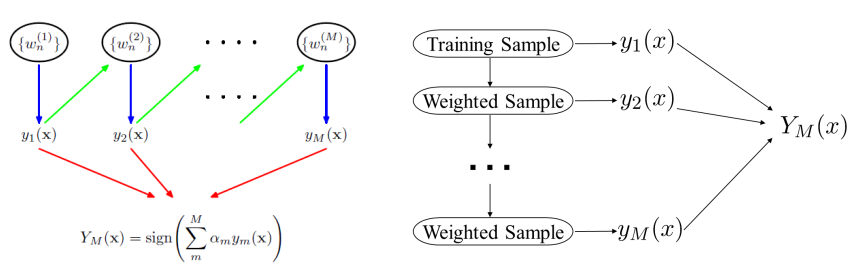
\includegraphics[width=.9\textwidth]{Boosting}
\end{center}


\(t_n\in\{-1,1\}, y(\bx)\in\{-1,1\}\)
.algorithm
\begin{enumerate}
\item initialize \(\{w_n\}\) by \(w_n^{(1)}=1/N\) for \(n=1,\dots,N\)
\item for \(m=1,\dots,M\)
\begin{enumerate}
\item find a classifier \(y_m(\bx)\) by minimizing 
\begin{equation*}
J_m=\displaystyle\sum_{n=1}^Nw_n^{(w)}I(y_m(\bx_n)\neq t_n)
\end{equation*}
where \(I=1\) if \(y_m(\bx_n)\neq t_n\)
\item evaluate
\begin{equation*}
\epsilon_m=J_m/\displaystyle\sum_{n=1}^Nw_n^{(m)}
\end{equation*}
then
\begin{equation*}
\alpha_m=\ln\lb\frac{1-\epsilon_m}{\epsilon_m}\rb
\end{equation*}
\item update
\begin{equation*}
w_n^{(m+1)}=w_n^{(m)}\exp\lb\alpha_mI(y_m(\bx_n)\neq t_n)\rb
\end{equation*}
\end{enumerate}
\item make prediction
\begin{equation*}
Y_M(\bx)=\text{sign}\left(\displaystyle\sum_{m=1}^M
\alpha_my_m(\bx)\right)
\end{equation*}
\end{enumerate}
\section{unsupervised learning - clustering em and PCA}
\label{sec:org9ffd32c}
\subsection{K-means clustering}
\label{sec:orga6a06e7}
use \(\bmu_k\) as a prototype associated with the \(k^{th}\) cluster, 
Distortion measure(responsibilities)
\(J=\displaystyle\sum_{n=1}^N \displaystyle\sum_{k=1}^Kr_{nk}
   \norm{\bl{x}_n-\bl{\mu}_k}^2\).

\begin{align*}
&\frac{\partial J}{\partial \bmu_k}=2 \displaystyle\sum_{n=1}^Nr_{nk}(\bx_n-\bmu_k)=0\\
&\bmu_k=\frac{\displaystyle\sum_nr_{nk}\bx_n}{\displaystyle\sum_{n}r_{nk}}\\
&r_{nk}=
\begin{cases}
1&\text{if } k=\arg\min_j\norm{\bx_n-\bmu_j}^2\\
0&\text{otherwise}
\end{cases}
\end{align*}

example: 5 data points and 3 clusters
\[
r_{n,k}=\begin{pmatrix}
 1 & 0 & 0 \\
 0 & 0 & 1 \\
 0 & 1 & 0 \\
 0 & 0 & 1 \\
 1 & 0 & 0 \\
\end{pmatrix}
\]

K-means algorithm (batch version):
\begin{enumerate}
\item Pick number of clusters k
\item Randomly scatter k “cluster centers” in data space
\item Repeat:
a. Assign each data point to its closest cluster center
b. Move each cluster center to the mean of the points assigned to it
\end{enumerate}


online k-means algorithm(sequential k-means)
\begin{equation*}
\bmu_k^{new}=\bmu_k^{old}+\eta_n(\bx_n-\bmu_k^{old})
\end{equation*}


k-medoids algorithm
\begin{itemize}
\item choose input daa points as center
\item Works with an arbitrary matrix of distances between data points instead of
Euclidean distance 
\begin{itemize}
\item E.g. Manhattan distance or Minkowski distance
\end{itemize}
\end{itemize}


\begin{equation*}
J=\displaystyle\sum_{n=1}^N \displaystyle\sum_{k=1}^Kr_{nk}
\norm{\bl{x}_n-\bl{\mu}_k}^2\Rightarrow
\widetilde{J}=\displaystyle\sum_{n=1}^N \displaystyle\sum_{k=1}^Kr_{nk}
\mathcal{V}(\bx_n,\bmu_k)
\end{equation*}


The limitation of K-means clustering
\begin{enumerate}
\item The K-means algorithm often convergence to a local minimum
\item The K-means algorithm adopts the hard assignment and doesn’t consider the
data density and probabilistic distribution.
\end{enumerate}
\subsection{Mixtures of Gaussians}
\label{sec:org3fbeea4}
\begin{itemize}
\item Definition: 
\begin{equation*}
p(\bl{x})=\displaystyle\sum_{k=1}^K\pi_k\mathcal{N}
(\bl{x}|\bl{\mu}_k,\bl{\Sigma}_k)\quad \displaystyle\sum_{k=1}^k\pi_k=1
\quad 0\le\pi_k\le1
\end{equation*}
\item introduce a K-dimensional binary random variable \(\bl{z}=(z_1,\dots,z_k)^T\)
\begin{equation*}
z_k\in\{0,1\}\quad \displaystyle\sum_kz_k=1\quad p(z_k=1)=\pi_k
\end{equation*}

Hence \(p(\bl{z})
     =\displaystyle\prod_{k=1}^K\pi_k^{z_k}\), \(\bz\) is \textbf{latent variable} (inferred
from other observed variables)

If \(p(\bl{x}|z_k=1)=\mathcal{N}(\bl{x}|\bl{\mu}_k,\bl{\Sigma})\), then
\(p(\bl{x}|\bl{z})=\displaystyle\prod_{k=1}^K\mathcal{N}(\bl{x}|\bl{\mu}_k,
     \bl{\Sigma}_k)^{z_k}\)
\item \textbf{equivalent formulation} of the Gaussian mixture.
\begin{align*}
\Aboxed{
p(\bl{x})&=\displaystyle\sum_{\bl{z}}p(\bl{x}|\bl{z})p(\bl{z})
=\displaystyle\sum_{\bl{z}}\displaystyle\prod_{k=1}^K
\mathcal{N}(\bl{x}|\bl{\mu}_k,\bl{\Sigma}_k)^{z_k}}\\
&=\displaystyle\sum_{j=1}^K\displaystyle\prod_{k=1}^K\mathcal{N}(\bl{x}|\bl{\mu}_k,
\bl{\Sigma}_k)^{I_{kj}}\quad I_{kj}=
\begin{cases}
1&\text{if } k=j\\
0&\text{otherwise}
\end{cases}\\
&=\displaystyle\sum_{j=1}^K\pi_j\mathcal{N}(\bl{x}|\bl{\mu}_j,\bl{\Sigma}_j)
\end{align*}

responsibility:
\begin{equation*}
\gamma(z_k)=p(z_k=1|\bx)=\frac{p(z_k=1)p(\bx|z_k=1)}{\dissum_{j=1}^Kp(z_j=1)p(\bx|z_j=1)}
=\frac{ \pi_k\caln(\bx|\bmu_k,\bSigma)}{\dissum_{j=1}^K\pi_j\caln(\bx|\bmu_j
\bSigma_j)}
\end{equation*}
\begin{center}
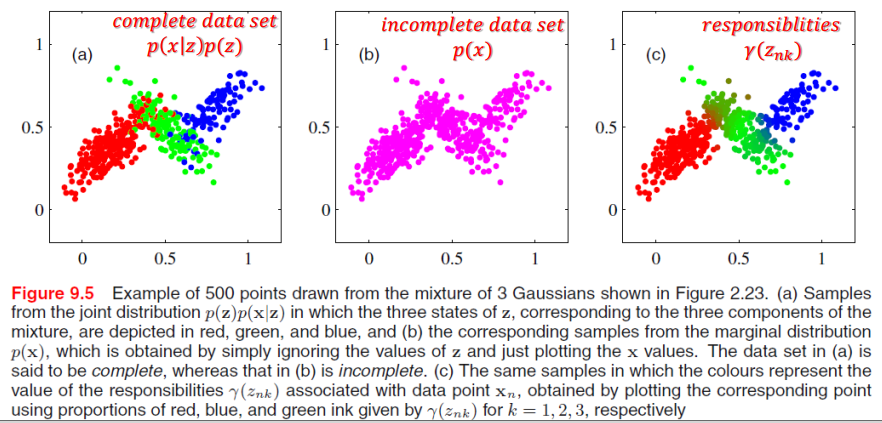
\includegraphics[width=.9\textwidth]{GMM}
\end{center}
\end{itemize}


\begin{equation*}
\ln p(\bX|\pi,\bmu,\bSigma)=\displaystyle\sum_{n=1}^N
\ln\lb \displaystyle\sum_{k=1}^K\pi_k\mathcal{N}(\bx_n|\bmu_k,
\bSigma_k)\rb
\end{equation*}
The difficulty of estimating parameters in GMM by ML
\begin{enumerate}
\item singularities

Collapses onto a specific data point
\item identifiability

Total K! equivalent solutions
\item no closed form solution

The derivatives of the log likelihood are complex
\end{enumerate}

\textbf{Expectation-Maximization algorithm for GMM}. 


\(p(\bX|)=\dispro p(\bx)\)

\(\ln p(\bX|\pi,\bmu, \bSigma)=\dissum_{n=1}^N\ln\left\{
   \dissum_{k=1}^K\pi_k\caln(\bx_n|\bmu_k,\bSigma_k)\right\}\)
\begin{enumerate}
\item E step
\begin{equation*}
\gamma(z_{nk})=\frac{\pi_k\caln(\bx_n|\bmu_k,\bSigma_k)}
{\dissum_j\pi_j\caln(\bx_n|\bmu_j,\bSigma_j)}
\end{equation*}
\item M step
\begin{itemize}
\item solve \(\bmu_k\)
\begin{align*}
&\frac{\partial\ln p(\bX|\pi,\bmu,\bSigma)}{\partial\bmu_k}=0\\
&0=-\displaystyle\sum_{n=1}^N\frac{\pi_k\caln(\bx_n|\bmu_k,\bSigma_k)}
{\dissum_j\pi_j\caln(\bx_n|\bmu_j,\bSigma_j)}\bSigma_k^{-1}(\bx_n-\bmu_k)\\
&\bmu_k=\frac{1}{N_k}\dissum_{n=1}^N\gamma(z_{nk})\bx_n\\
&N_k=\dissum_{n=1}^N\gamma(z_{nk})
\end{align*}
\item solve \(\bSigma_k\)
\begin{align*}
&\frac{\partial\ln p(\bX|\pi,\bmu,\bSigma)}{\partial\bSigma_k}=0\\
&\bSigma_k=\frac{1}{N_k}\dissum_{n=1}^N\gamma(z_{nk})(\bx_n-\bmu_k)(\bx_n-\bmu_k)^T
\end{align*}
\item solve \(\pi_k\)
\begin{align*}
&\frac{\partial}{\partial\pi_k}\lb\ln p(\bX|\pi,\bmu,\bSigma)
+\lambda\left (\displaystyle\sum_{k=1}^K\pi_k-1\right)\rb=0\\
&0=\displaystyle\sum_{n=1}^N\frac{\caln(\bx_n|\bmu_k,\bSigma_k)}
{\sum_j\pi_j\caln(\bx_n|\bmu_j,\bSigma_j)}+\lambda\\
&\pi_k=\frac{N_k}{N}
\end{align*}
\end{itemize}
\end{enumerate}


\textbf{EM for Gaussian Mixtures}
\begin{enumerate}
\item initialize the means \(\bmu_k\), covariances \(\bSigma_k\) and mixing
coefficients \(\pi_k\)
\item E step

find the posterior probability of latent variable

\begin{equation*}
\gamma(z_{nk})=\frac{\pi_k\caln(\bx_n|\bmu_k,\bSigma_k)}
{\dissum_j\pi_j\caln(\bx_n|\bmu_j,\bSigma_j)}
\end{equation*}
\item M step
\begin{align*}
&\bmu_k^{new}=\frac{1}{N_k}\dissum_{n=1}^N\gamma(z_{nk})\bx_n\\
&\bSigma_k^{new}=\frac{1}{N_k}\dissum_{n=1}^N\gamma(z_{nk})(\bx_n-
\bmu_k^{new})(\bx_n-\bmu_k^{new})^T\\
&\pi_k^{new}=\frac{N_k}{N}\quad \text{where }
N_k=\displaystyle\sum_{n=1}^N
\gamma(z_{nk})\\
\end{align*}
\item evaluate the log likelihood
\begin{equation*}
\ln p(\bX|\pi,\bmu, \bSigma)=\dissum_{n=1}^N\ln\left\{
\dissum_{k=1}^K\pi_k\caln(\bx_n|\bmu_k,\bSigma_k)\right\}
\end{equation*}
and check for convergence of either the parameters or the log likelihood.
If the convergence criterion is not satisfied return to step 2
\end{enumerate}
\subsection{An alternative view of EM}
\label{sec:orgbf3f04a}
\subsubsection{the general EM algorithm}
\label{sec:orged90c52}

Data \(\bX\), observation \(\btheta\)
The log likelihood of a discrete latent variables model
\begin{equation*}
\ln p(\bX|\btheta)=\ln\lb \displaystyle\sum_{\bZ} p(\bX,\bZ|\btheta)\rb
\end{equation*}


\emph{the goal of EM algorithm is to find maximum likelihood solution for models
having latent variables} 


For the complete data set \(\lb\bX,\bZ\rb\), the likelihood function
\begin{equation*}
\ln p(\bX|\btheta)\Longrightarrow \ln p(\bX,\bZ|\btheta)
\end{equation*}


For the incomplete data set \(\lb\bX\rb\), we adopt the following steps to
find maximum likelihood solution

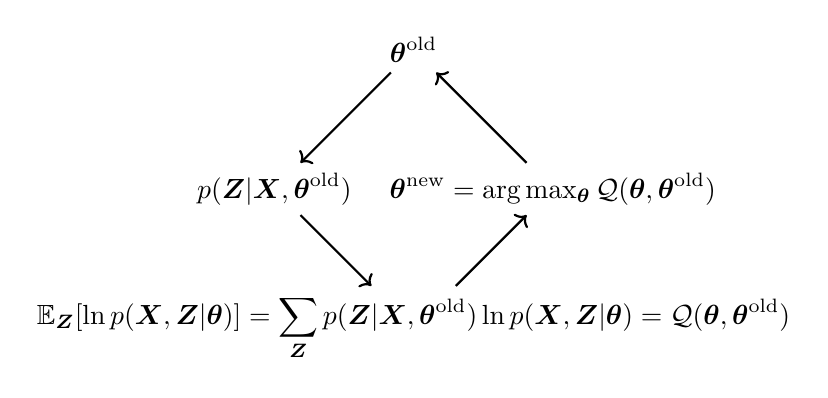
\begin{tikzpicture}[node distance=2.5cm]
\tikzstyle{arrow}=[->,thick];
\node (1) [] {$\btheta^\text{old}$};
\node (2) [below left of=1] {$p(\bZ|\bX,\btheta^\text{old})$};
\node (3) [below right of=2] {$\E_{\bZ}[\ln p(\bX,\bZ|\btheta)]=\displaystyle\sum_{\bZ}
p(\bZ|\bX,\btheta^\text{old})\ln p(\bX,\bZ|\btheta)=\calq (\btheta,\btheta^\text{old})$};
\node (4) [below right of=1] {$\btheta^\text{new}=\text{arg} \max_{\btheta}\calq(\btheta,\btheta^\text{old})$};
\draw [arrow] (1) -- (2);
\draw [arrow] (2) -- (3);
\draw [arrow] (3) -- (4);
\draw [arrow] (4) -- (1);
\end{tikzpicture}

the general EM algorithm

Given a joint distribution \(p(\bX, \bZ|\btheta)\) over observed variables
\(\bX\) and latent variables \(\bZ\), govened by parameters \(\btheta\), the goal
is to maximize the likelihood function \(p(\bX|\btheta)\)
\begin{enumerate}
\item choose an initial setting for the parameters \(\btheta^{old}\)
\item \textbf{E step} evaluate \(p(\bZ|\bX,\btheta^{old})\)
\item \textbf{M step} 
\begin{align*}
&\btheta^\text{new}=\text{arg} \max_{\btheta}\calq(\btheta,\btheta^\text{old})\\
&\calq (\btheta,\btheta^\text{old})=
\displaystyle\sum_{\bZ}p(\bZ|\bX,\btheta^\text{old})\ln p(\bX,\bZ|\btheta)\\
&\calq(\btheta,\btheta^{old}+\ln p(\btheta))
\end{align*}
\item check for convergence of either the log likelihood or the parameter
values. If the convergence criterion is not satisfied, then let
\begin{equation*}
\btheta^{old}\leftarrow \btheta^{new}
\end{equation*}
\end{enumerate}
\subsubsection{Gaussian mixtures revisited}
\label{sec:orgc59c149}
\begin{align*}
&p(\bX,\bZ|\bmu,\bSigma,\pi)=\displaystyle\prod_{n=1}^N
\displaystyle\prod_{k=1}^K\pi_k^{z_{nk}}\caln(\bx_n|\bmu_k,\bSigma_k)^{z_{nk}}\\
&\ln p(\bX,\bZ|\bmu,\bSigma,\pi)=\displaystyle\sum_{n=1}^N
\displaystyle\sum_{k=1}^Kz_{nk}\lb\ln\pi_k+\ln\caln(\bx_n|\bmu_k,\bSigma_k)\rb\\
&\pi_k=\frac{1}{N}\displaystyle\sum_{n=1}^Nz_{nk}\\
&\E_{\bZ}[\ln p(\bX,\bZ|\bmu,\bSigma,\pi)]=\displaystyle\sum_{n=1}^N
\displaystyle\sum_{k=1}^K\gamma(z_{nk})\lb\ln\pi_k+
\ln\caln(\bx_n|\bmu_k,\bSigma_k)\rb\\
\end{align*}


relation to K-means
\subsection{The EM in general}
\label{sec:org359b73a}
\subsection{PCA}
\label{sec:org0037092}
dimensionality reduction: The result of Dimensionality reduction should keep
the original data structure

\begin{align*}
&\text{Var}(X)=\frac{1}{n}\displaystyle\sum_{i=1}^n(x_i-\bar{x})^2\\
&\text{cov}{X,Y}=\frac{1}{n}\displaystyle\sum_{i=1}^n(x_i-E(X))(y_i-E(Y))\\
&\text{corr(X,Y)}=\frac{\text{cov}(X,Y)}{\sqrt{\text{Var}(X)\text{Var}(Y)}}
=\frac{\text{Cov}(X,Y)}{\sigma_x\sigma_y}\\
\end{align*}
Pearson correlation coefficients
\begin{enumerate}
\item \(\abs{corr(X,Y)}\le 1\)
\item \(corr(X,Y)=1\leftrightarrow\exists a,b,Y=aX+b\)
\item Pearson Correlation coefficient measures the degree of linear correlation
between variable X and Y
\item Positive correlation means as X increases, so does Y. Negative correlation
means as X increases, Y goes down
\end{enumerate}


motivation:
\begin{enumerate}
\item In dimension reduction, data should be projected to the direction with
the largest variance as far as possible, by this way the information
contained in the data is preserved and the personality is highlighted.
\item The motivation of PCA is to project d-dimensional data to l-dimensional
space(\(d\gg l\)) and remove the redundancy between data( by removing
correlation between data).
\end{enumerate}


Given \(D=\{\bx_1,\dots,\bx_n\}, \bx_i\in\R^d\), then
\begin{equation*}
\bY_{n\times l}=\bX_{n\times d} \bW_{d\times l}
\end{equation*}
\begin{align*}
&var(\bY)=\frac{1}{n}trace(\bY^T\bY)=\frac{1}{n}trace(\bW^T\bX^T
\bX\bW)=trace(\bW\frac{1}{n}\bX^T\bX\bW)\\
&\Sigma=\frac{1}{n}\bX^T\bX\\
&\max_{\bW}trace(\bW^T\bSigma\bW), \bw_i^T\bw_i=1,i\in\{1,\dots,l\}
\end{align*}

Use Lagrangian multiplier
\begin{equation*}
L(\bW,\blambda)=trace(\bW^T\bSigma\bW)-\displaystyle\sum_{i=1}^l
\lambda_i(\bw_i^T\bw_i^T-1)
\end{equation*}
by partial derivative, we get
\begin{equation*}
\bSigma\bw_i=\lambda_i\bw_i
\end{equation*}
\begin{equation*}
trace(\bW^T\bSigma\bW)=\displaystyle\sum_{i=1}^l\lambda_i
\end{equation*}

algorithm
\begin{enumerate}
\item centralization \(\bx_i=\bx_i-\bar{\bx}\)
\item \(\bSigma=\frac{1}{n}\bX^T\bX\)
\item get the eigenvalues of \(\bSigma\) and sort
\begin{equation*}
\lambda_1\ge \lambda_2\ge\dots\ge \lambda_1
\end{equation*}
\item Select the eigenvectors corresponding to top l biggest eigenvalues to form
mapping matrix \(\bW\)
\item Reduce the dimension of every sample \(\bx_i\)
\begin{equation*}
(\bx_i)_{1\times d}\bW_{d\times l}=1\times l
\end{equation*}
\end{enumerate}
\section{deep learning}
\label{sec:orgbf5cbbc}
\subsection{Neural networks}
\label{sec:org17b06c2}
\subsubsection{biological inspiration}
\label{sec:org73b1184}
activation functions(non-linear functions)
\begin{itemize}
\item sigmoid/logistic, tanh, rectified linear unit(ReLu)
\end{itemize}


\begin{center}
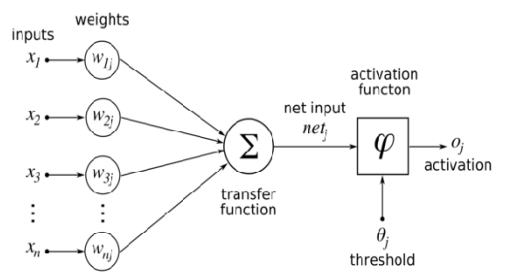
\includegraphics[width=.9\textwidth]{ActivationFunction}
\end{center}


\begin{center}
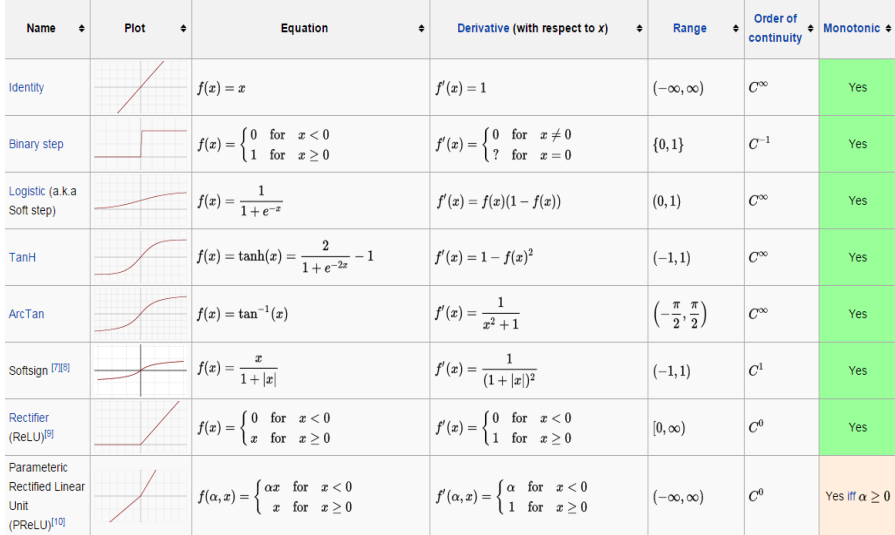
\includegraphics[width=.9\textwidth]{activation}
\end{center}

\subsubsection{feedforward NN}
\label{sec:org84bea6c}
\textbf{fully-connected layer}: neurons between two adjacent layers are fully
pairwise connected
\begin{center}
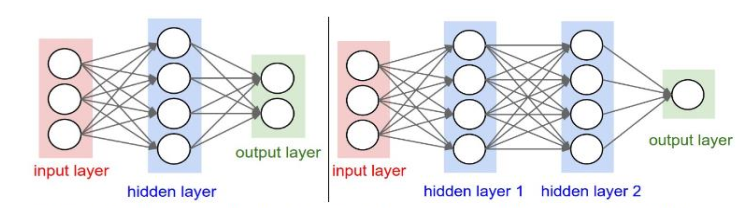
\includegraphics[width=.9\textwidth]{FeedForwardNN}
\end{center}

perception networks: Single-layer feed-forward neural networks (no hidden
units) 
\begin{center}
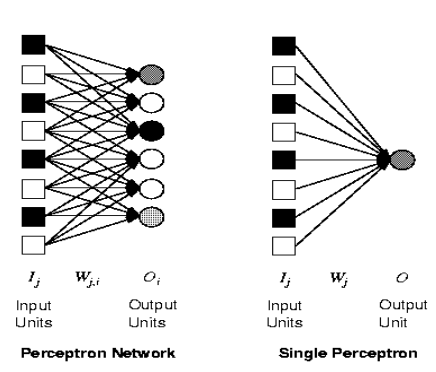
\includegraphics[width=.9\textwidth]{Perceptron}
\end{center}


Given any continuous function \(f(x)\) and some \(\epsilon<0\), there exists a
Neural network \(g(x)\) with one hidden layer s.t. 
\begin{equation*}
\forall x, \abs{f(x)-g(x)}<\epsilon
\end{equation*}

We increase the size and number of layers in a Neural Network, the \textbf{capacity}
of the network increases. That is, the space of representable functions
grows since the neurons can collaborate to express many different functions
\subsection{optimization and gradient descent}
\label{sec:org8f73b6d}
Problem: how to lean the best W of a classifier
\begin{itemize}
\item dataset \((x,y)\)
\item score function \(s=f(x;W)=Wx\)
\item loss function
\begin{itemize}
\item softmax \(L_i=-\log(\frac{e^{s_{y_i}}}{\sum_je^{s_j}})\)
\item SVM \(L_i=\sum_{j\neq y_i}\max(0,s_j-s_{y_i}+1)\)
\item full loss \(L=\frac{1}{N}\displaystyle\sum_{i=1}^NL_i+R(W)\)
\end{itemize}
\end{itemize}
\subsubsection{gradient descent}
\label{sec:orgd3cef8b}
\subsubsection{stocahstic gradient descent}
\label{sec:org726357d}
\begin{align*}
&L(W)=\frac{1}{N}\displaystyle\sum_{i=1}^NL_i(x_i,y_i,W)+\lambda R(W)\\
&\nabla_WL(W)=\frac{1}{N}\displaystyle\sum_{i=1}^N\nabla_WL_i(x_i,y_i,W)
+\lambda\nabla_WR(W)
\end{align*}

Approximate sum using a \textbf{minibatch} of examples
\subsubsection{backpropagation}
\label{sec:orgeb539ba}
computation graph
\begin{center}
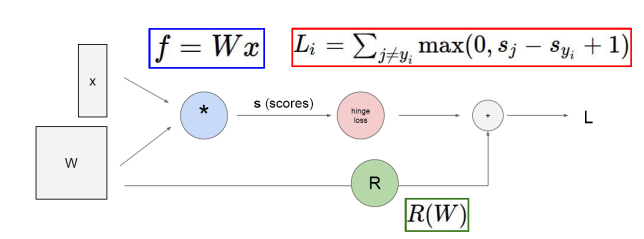
\includegraphics[width=.9\textwidth]{ComputationalGraph}
\end{center}


\textbf{Forward computation}
\begin{center}
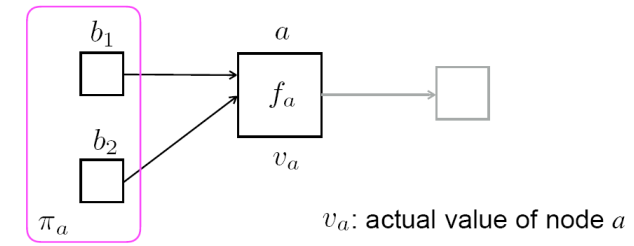
\includegraphics[width=.9\textwidth]{ForwardComputation}
\end{center}
\begin{itemize}
\item Each node represented as a variable \(a\)
\item \(v_a=f_a(v_{b_1},\dots,v_{b_m})\)
\end{itemize}


\textbf{Backward computation}
\begin{center}
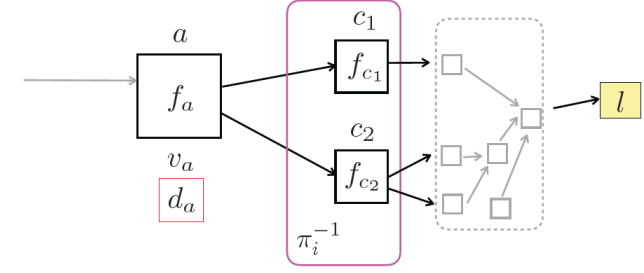
\includegraphics[width=.9\textwidth]{BackwardComputation}
\end{center}
\begin{itemize}
\item \(d_a=\frac{\partial l}{\partial a}\)
\item In general, \(d_a=\displaystyle\sum_{c_i\in\pi_a^{-1}}d_{c_i}\cdot
      \frac{\partial f_{c_i}}{\partial a}\)
\item In this case, \(d_a=d_{c_1}\frac{\partial f_{c_1}}{\partial a}+
      d_{c_2}\frac{\partial f_{c_2}}{\partial a}\)
\end{itemize}


\begin{center}
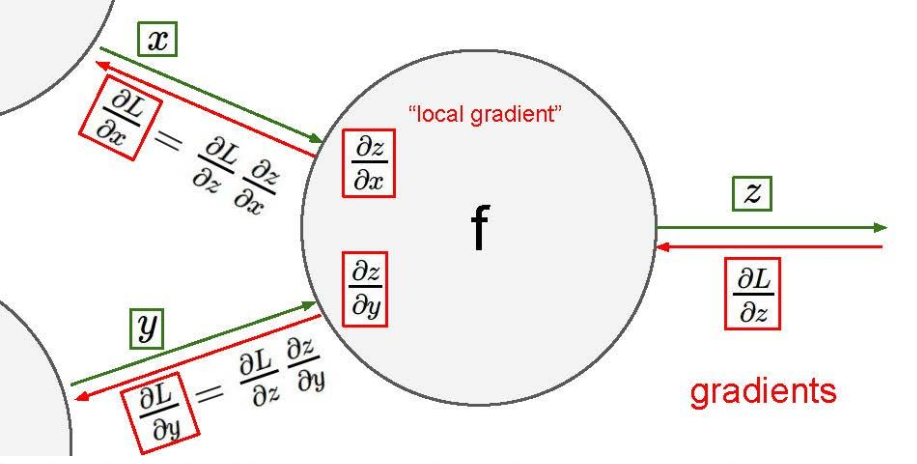
\includegraphics[width=.5\textwidth]{Backpro}
\end{center}


\begin{equation*}
\frac{d\sigma(x)}{dx}=(1-\sigma(x))\sigma(x)
\end{equation*}


patterns in backward flow
\begin{itemize}
\item \textbf{add} gate: gradient distributor
\item \textbf{max} gate: gradient router
\item \textbf{mul} gate: gradient switcher
\end{itemize}


For gradients for vectorized code, \(\frac{\partial \bz}{\partial\bx}\) is
\textbf{Jacobian matrix}. For example, \(f(x,W)=\norm{W\cdot}^2=\sum_{i=1}^n(W\cdot
    x)^2_i\)

\begin{center}
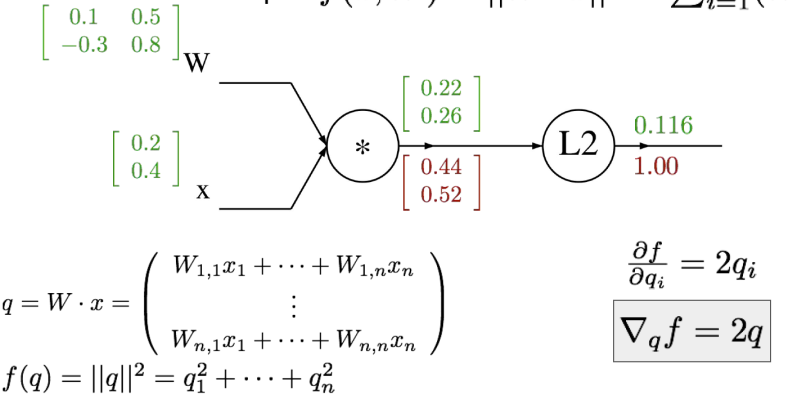
\includegraphics[width=.9\textwidth]{Backpro1}
\end{center}
\begin{center}
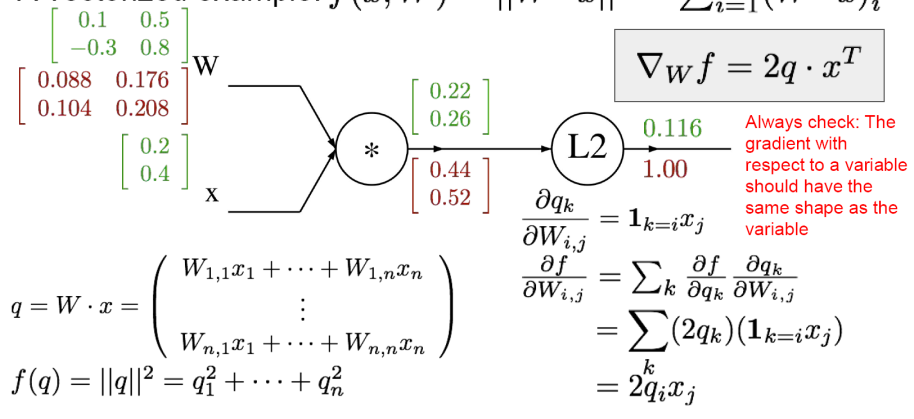
\includegraphics[width=.9\textwidth]{Backpro2}
\end{center}
\begin{center}
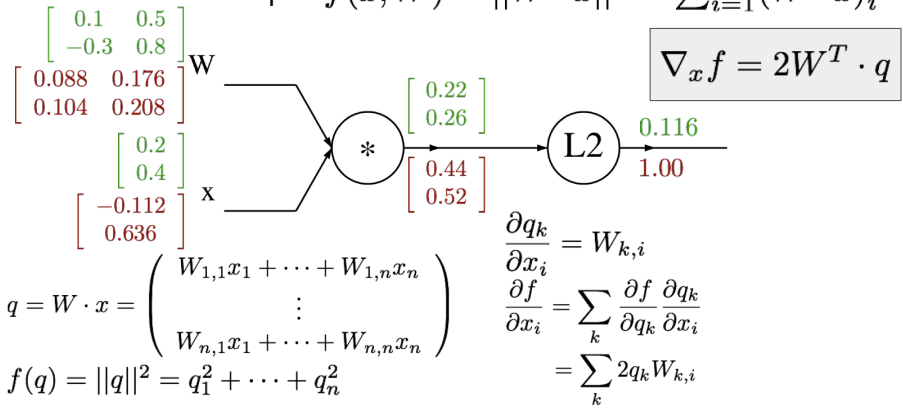
\includegraphics[width=.9\textwidth]{Backpro3}
\end{center}

\subsection{convolutional neural network}
\label{sec:org2427f23}
\subsubsection{basic concepts}
\label{sec:org1aed530}
summary:
\begin{itemize}
\item accepts a volume of size \(W_1\times H_1\times D_1\)
\item four hyperparameters
\begin{itemize}
\item number of filters K
\item their spatial extent F
\item the stride S
\item the amount of zero padding P
\end{itemize}
\item produces a volume of size \(W_2\times H_2\times D_2\)
\begin{itemize}
\item \(W_2=(W_1-F+2P)/S+1\)
\item \(H_2=(H_1-F+2P)/S+1\)
\item \(D_2=K\)
\end{itemize}
\item parameter: \(F^2\times D_1\times K+K\)
\end{itemize}


Pooling layer
\begin{itemize}
\item Its function is to progressively reduce the spatial size of the
representation to reduce the amount of parameters and computation in the
network, and hence to also control overfitting
\item The Pooling Layer operates independently on every depth slice of the input
and resizes it spatially, using the MAX operation
\end{itemize}


Normalization layer
\begin{itemize}
\item Many types of normalization layers have been proposed for use in ConvNet
architectures, sometimes with the intentions of implementing inhibition
schemes observed in the biological brain. However, these layers have
recently fallen out of favor because in practice their contribution has
been shown to be minimal, if any.
\end{itemize}


Fully-connected layer
\begin{itemize}
\item Neurons in a fully connected layer have full connections to all
activations in the previous layer, as seen in regular Neural Networks.
Their activations can hence be computed with a matrix multiplication
followed by a bias offset.
\item Any FC layer can be converted to a CONV layer
\item By converting FC layers to CONV layers, we can build a Fully Convolutional
Networks
\end{itemize}
\subsubsection{case study: AlexNet, GoogLeNet, VGG}
\label{sec:org975622b}

\subsection{Appication of deep learning}
\label{sec:orgcf08656}

\subsection{Recurrent Neural Network(RNN)}
\label{sec:org31ded1b}
\subsubsection{RNN}
\label{sec:org2cffb5f}
A family of neural networks for \textbf{processing sequential data} 
\(x^{(1)},x^{(2)},\dots,x^{(\tau)}\)
\begin{center}
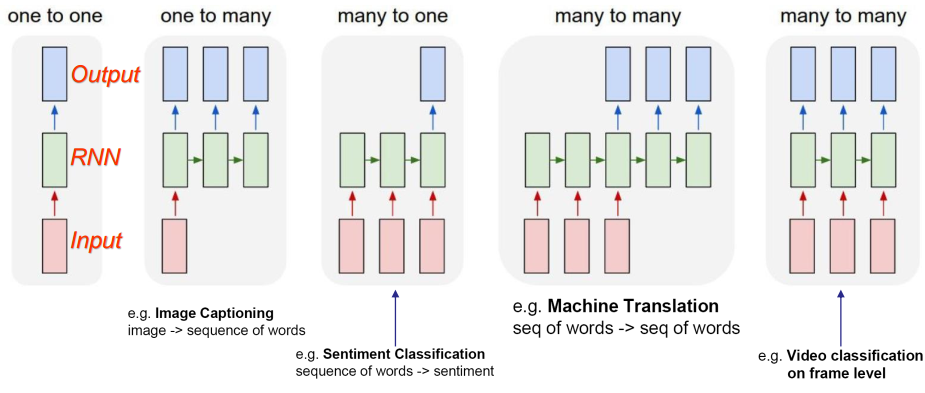
\includegraphics[width=.9\textwidth]{RNNsequential}
\end{center}

\begin{center}
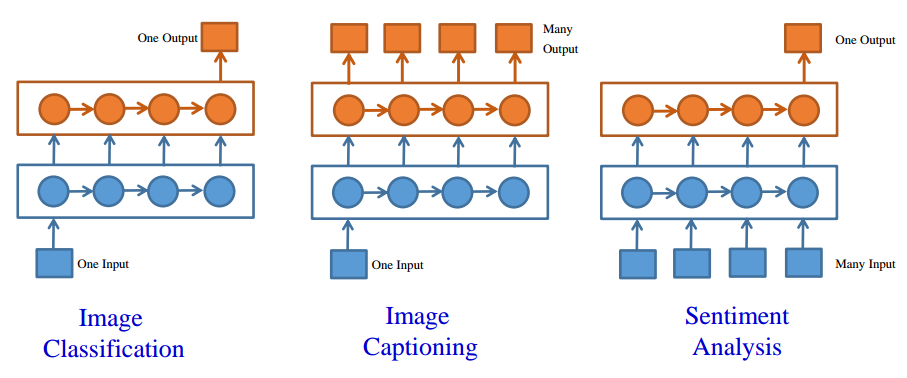
\includegraphics[width=.9\textwidth]{Seq2seq1}
\end{center}
\begin{center}
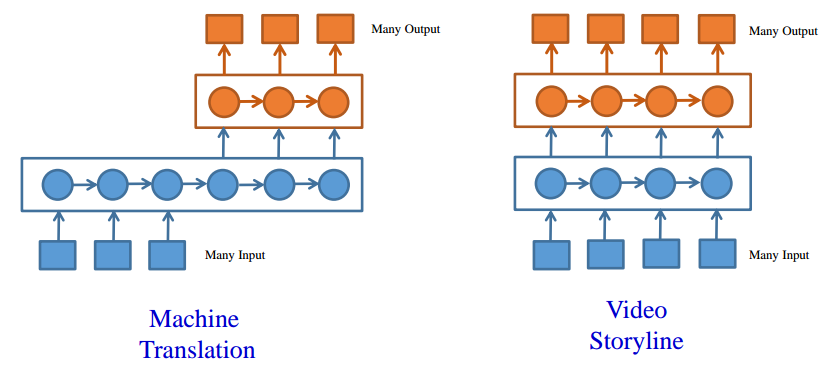
\includegraphics[width=.9\textwidth]{Seq2seq2}
\end{center}


Vanilla RNN
\begin{align*}
&h_t=f_W(h_{t-1},x_t)\\
&h_t=\tanh(W_{hh}h_{t-1}+W_{xh}x_t)\\
&y_t=W_{hy}h_t\\
&y_t=\text{softmax}(W_{hy}h_t)
\end{align*}


\begin{center}
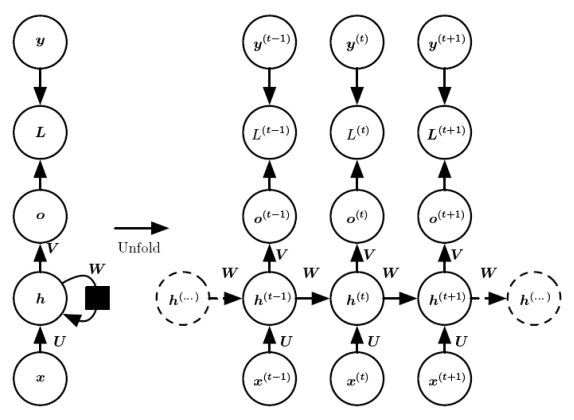
\includegraphics[width=.9\textwidth]{RNNGraph}
\end{center}
\begin{align*}
&\ba^{(t)}=\bb+\bW\bh^{(t-1)}+\bU\bx^{(t)}\\
&\bh^{(t)}=\tanh(\ba^{(t)})\\
&\bo^{(t)}=\bc+\bV\bh^{(t)}\\
&\hat{\by}^{(t)}=\text{softmax}(\bo^{(t)})
\end{align*}

\begin{equation*}
L(\lb \bx^{(1)},\dots,\bx^{(\tau)}\rb,\lb\by^{(1)},\dots,\by^{(\tau)} \rb)=
\displaystyle\sum_tl^{(t)}=-\displaystyle\sum_t\log p_{model}
(y^{(t)}|\lb\bx^{(1)},\dots,\bx^{(t)}\rb)
\end{equation*}


Training a RNN with gradient flow
\begin{center}
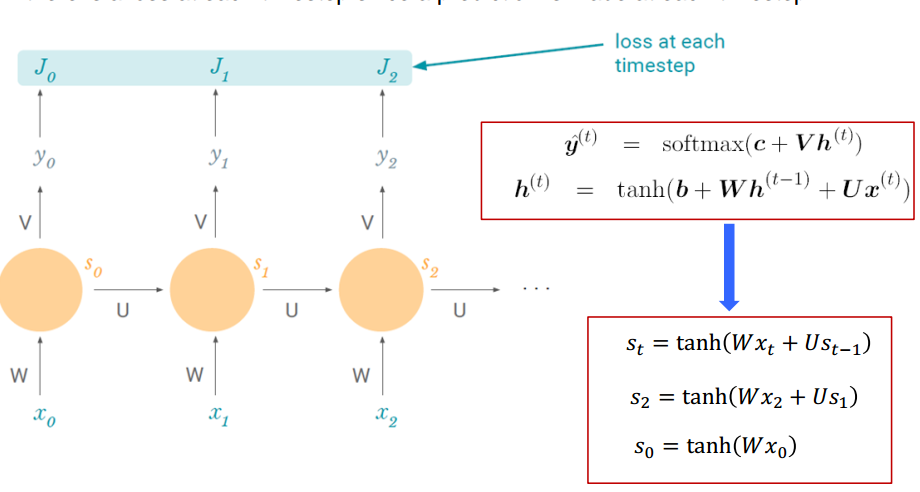
\includegraphics[width=.9\textwidth]{RNNback}
\end{center}
loss at time \(t=J_t(\bTheta)\), total loss \(J(\bTheta)=\sum_tJ_t(\bTheta)\)
hence
\begin{equation*}
\frac{\partial J}{\partial P}=\displaystyle\sum_t\frac{\partial J_t}{\partial P}
\end{equation*}
\begin{align*}
&\frac{\partial J_2}{\partial W}=\frac{\partial J_2}{\partial y_2}\frac{\partial y_2}
{\partial s_2}\frac{\partial s_2}{\partial W}\\
&s_2=\tanh(Us_1+Wx_2)\\
&\frac{\partial J_t}{\partial W}=\displaystyle\sum_{k=0}^t
\frac{\partial J_t}{\partial y_t}\frac{\partial y_t}
{\partial s_t}\frac{\partial s_t}{\partial s_k}
\frac{\partial s_k}{\partial W}\\
\end{align*}

Hard to train
\subsubsection{long short-term memory and other gated RNNs}
\label{sec:orga002546}
\begin{center}
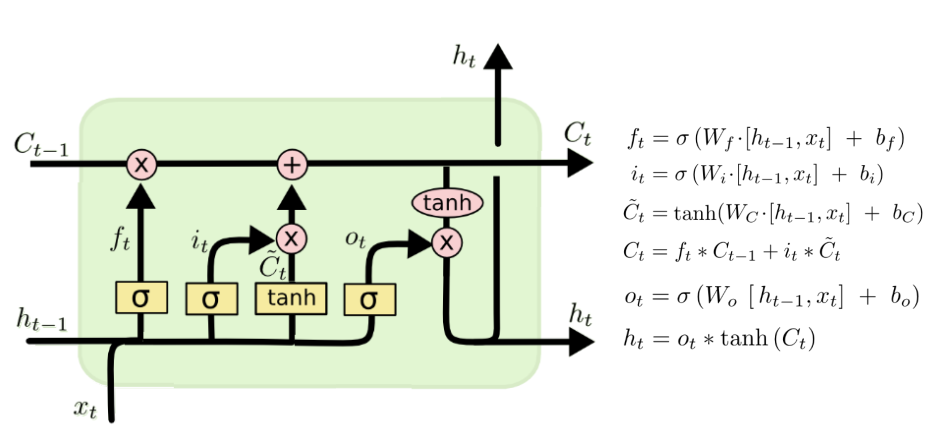
\includegraphics[width=.9\textwidth]{LSTM}
\end{center}

\section{reinforcement learning}
\label{sec:orgfc29cb8}
\subsection{About RL}
\label{sec:org511043b}
RL addresses the question of how an autonomous agent that sense and acts in
its environment can learn an optimal control strategy, or policy, for
choosing actions to achieve its goals (maximize cumulative reward).


A \textbf{reward} \(R_t\) is a scalar feedback signal. The agent’s job is to maximize
cumulative reward 

\textbf{Reward hypothesis}: All goals can be described by the maximization of expected
cumulative reward 

At each step \(t\) the agent
\begin{itemize}
\item Receives observation \(O_t\)
\item Executes action \(A_t\)
\item Receives scalar reward \(R_t\)
\end{itemize}


the environment:
\begin{itemize}
\item Receives action \(A_t\)
\item Emits scalar reward \(R_{t+1}\)
\item Emits observation \(O_{t+1}\)
\end{itemize}


\begin{center}
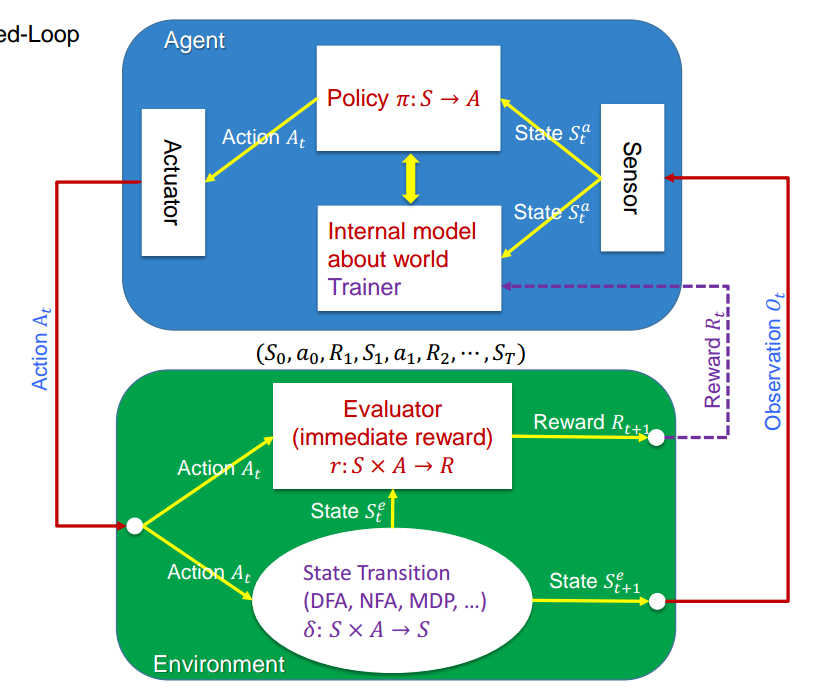
\includegraphics[width=.9\textwidth]{AgentEnv}
\end{center}

\textbf{policy}: agent's behaviour function.

\textbf{value function}: how good is each state

\textbf{model}: agent's representation of the environment
\begin{center}
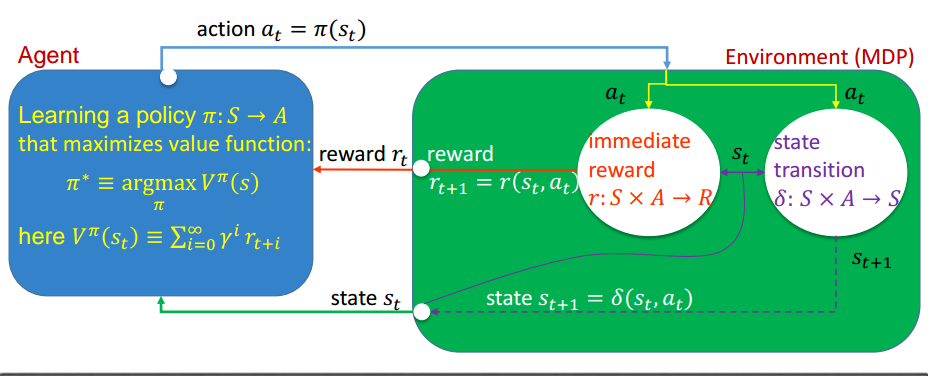
\includegraphics[width=.9\textwidth]{RLcomponent}
\end{center}

History is the sequence of observations, actions, rewards
\begin{equation*}
H_t=O_1,A_1,R_1,\dots,O_t,A_t,R_t
\end{equation*}
\subsection{Markov Decision processes}
\label{sec:orga598e30}
\begin{definition}
A state $S_t$ is \textbf{Markov} if and only if
\begin{equation*}
\P[S_{t+1}|S_t]=\P[S_{t+1}|S_1,\dots,S_t]
\end{equation*}
\end{definition}

\begin{definition}
A \textbf{Markov Process} is a tuple $<\cals,\calp>$
\begin{itemize}
\item $\cals$ is a (finite) set of states
\item $\calp$ is a state transition probability matrix
\begin{equation*}
\calp_{ss'}=\P[S_{t+1}=s'|S_t=s]
\end{equation*}
\end{itemize}
\end{definition}


\begin{definition}
A \textbf{Markov Reward Process} is a tuple $<\cals,\calp,\calr, \gamma>$
\begin{itemize}
\item $\cals$ is a (finite) set of states
\item $\calp$ is a state transition probability matrix
\begin{equation*}
\calp_{ss'}=\P[S_{t+1}=s'|S_t=s]
\end{equation*}
\item $\calr$ is a reward function, $\calr_s=\E[R_{t+1}|S_t=s]$
\item $\gamma$ is a discount factor, $\gamma\in[0,1]$
\end{itemize}
\end{definition}

\begin{definition}
The \textbf{return} $G_t$ is the total discounted reward from time-step $t$
\begin{equation*}
G_t=R_{t+1}+\gamma R_{t+2}+\dots=\displaystyle\sum_{k=0}^\infty\gamma^kR_{t+k+1}
\end{equation*}
\end{definition}
The \textbf{discount factor} \(\gamma\) is the present value of future rewards. The
value of receiving reward \(R\) after \(k+1\) time-steps is \(\gamma^kR\)

\begin{definition}
A \textbf{Markov Decision Process} is a tuple $<\cals, \cala,\calp,\calr,\gamma>$
\begin{itemize}
\item $\cals$ is a (finite) set of states
\item $\calp$ is a state transition probability matrix
\item $\cala$ is a finite set of actions
\begin{equation*}
\calp_{ss'}^a=\P[S_{t+1}=s'|S_t=s]
\end{equation*}
\item $\calr$ is a reward function, $\calr_s=\E[R_{t+1}|S_t=s]$
\item $\gamma$ is a discount factor, $\gamma\in[0,1]$
\end{itemize}
\end{definition}

\textbf{policy function} \(\pi:\cals\times\cala\to[0,1]\) 
\begin{itemize}
\item where the value of \(\pi(s,a)\) represents the probability of taking action
\(a\) under \(s\) 
\begin{itemize}
\item \textbf{stochastic} policy: \(\pi(a|s)=\P[A_t=a|S_t=s]=\P[a|s]\)
\item \textbf{deterministic} policy: \(a=\pi(s), a\in\cala\)
\end{itemize}
\end{itemize}


In order to evaluate policy function \(\pi\), define:
\begin{enumerate}
\item \textbf{value function} \(V:\cals\to\R\) where 
\begin{align*}
V_\pi(s)&=\E_\pi[G_t|S_t=s]\\
&=\E_\pi[R_{t+1}+\gamma R_{t+2}+\dots|S_t=s]\\
&=\E_{a\sim\pi(s,\cdot)}[\E_\pi[R_{t+1}+\gamma R_{t+2}+\dots|S_t=s,A_t=a]]\\
&=\displaystyle\sum_{a\in A}\pi(s,a)q_\pi(s,a)
\end{align*}
\item \textbf{Q-value function/ Action-value Function} \(q:\cals\times\cala\to\R\), where
\begin{align*}
q_\pi(s,a)&=\E_\pi[G_t|S_t=s,A_t=a]\\
&=\E_\pi[R_{t+1}+\gamma R_{t+2}+\dots|S_t=s,A_t=a]\\
&=\E_{s'\sim Pr(\cdot|s,a)}[R(s,a,s')+\gamma
\E_\pi[R_{t+2}+\gamma R_{t+3}+\dots|S_{t+1}=s]]\\
&=\displaystyle\sum_{s'\in S}Pr(s'|s,a)[R(s,a,s')+\gamma V_\pi(s')]
\end{align*}
\end{enumerate}
\subsection{policy improvement and policy evaluation}
\label{sec:org8fff090}
RL problem: given Markov decision process
\(MDP=\{\cals,\cala,\calr,\calp,\gamma\}\), find an optimal policy \(\pi^*\)
which maximizes the value of \(V_{\pi^*}(s)\) for any \(s\in\cals\)
\subsubsection{value-based solution method}
\label{sec:org83511fa}
\begin{enumerate}
\item policy improvement

let \(\pi,\pi'\) be any deterministic policies, for all \(s\in\cals\):
\begin{equation*}
q_\pi(s,\pi'(s))\ge q_\pi(s,\pi(s))
\end{equation*}
that is for all states \(s\in\cals\)
\begin{equation*}
V_{\pi'}(s)\ge V_\pi(s)
\end{equation*}
then \(\pi'\) must be as goog as, or better than \(\pi\)
\begin{equation*}
\pi'(s)=\arg\max_aq_\pi(s,a)\quad \text{for all } s\in\cals
\end{equation*}
\item policy evaluation

iterative calculation of bellman equation
\end{enumerate}
\subsection{q-learning for RL}
\label{sec:org6c1a952}
\section{wef}
\label{sec:org9a4416f}
\subsection{wfe}
\label{sec:orgb2dbae5}
K-means
\end{document}